\documentclass[a4paper,12pt]{report}

% input/text packages
\usepackage[utf8]{inputenc}
\usepackage[english]{babel}
\usepackage{amssymb}
\usepackage{calc}
\usepackage{siunitx}

% graphical/layout packages
\usepackage[top=1in, bottom=1.5in, left=1in, right=1in]{geometry}
\usepackage{graphicx, wrapfig}
\usepackage{booktabs}
\usepackage{subcaption}
\usepackage{float}
\usepackage{enumitem}
\usepackage{multicol}
\usepackage{rotating}
\setlist[itemize]{noitemsep, topsep=4pt}
\setlist[enumerate]{itemsep=0pt, topsep=4pt}

% setup biblatex/bibliography
\usepackage[
    backend=biber,
    style=ieee,
    sortlocale=en_UK,
    natbib=true,
    url=true,
    doi=true,
    eprint=true,
    autocite=superscript
]{biblatex}
\addbibresource{references.bib}
\makeatletter
\let\cite\supercite

%Set graphics path
\graphicspath{ {img/} }

\usepackage{xcolor}
\usepackage[colorlinks = true,
            linkcolor = blue,
            urlcolor  = blue,
            citecolor = blue,
            anchorcolor = blue]{hyperref}

\def\LTU{Luleå University of Technology}
\def\taiga{\href{https://taiga.io}{taiga.io}}
\def\techio{\href{https://tech.io}{tech.io}}
\def\sockr{\href{https://github.com/ArmedGuy/Sockr}{Sockr}}

\def\nodejs{Node.JS}


\begin{document}

\begin{titlepage}
    \begin{center}
    {\LARGE D7017E:\@ Report}\par
    \vspace{\baselineskip}

    {\Large Luleå Tekniska Universitet}\\{\large 971 87 Luleå, Sverige}\par
\end{center}

\vfill

\membergroup{Nils Fitinghoff}{Software Engineer \\ Tester, Backend}
            {Anton Jerhamre}{Software Engineer \\ Frontend}

\membergroup{David Sandström}{Software Engineer \\ Backend}
            {Mikael Hedkvist}{Software Engineer \\ Backend}

\membergroup{Henrik Nilsson Harnert}{Software Engineer \\ Tester, Backend}
            {Axel Sundbom}{Software Engineer \\ Tester, Frontend \\ Repository Maintainer \\ Hardware Maintainer}

\membergroup{Niklas Fuks}{Project Manager}
            {Tim Granström}{Software Engineer\\ Backend}

\membergroup{Christopher Rosenvall}{Software Engineer \\ Frontend}
            {Fredrik Bostrand}{Software Engineer \\ Backend}

\membergroup{Linn Danielsson}{Software Engineer \\ Frontend}
            {Tobias Axelsson}{Software Engineer \\ Backend}

\membergroup{Rickard Nordlander}{Software Engineer \\ Tester, Frontend}
            {Axel Vallin}{Software Engineer \\ Frontend}


\begin{center}
    \begin{member}
    \centering
    Anders Mikkelä\par
    \spacerule{\widthof{Anders Mikkelä}}
    Frontend
    \end{member}
\end{center}

\vfill

\begin{center}
    Supervised by\\ Peter Parnes
\end{center}

\end{titlepage}

 \begin{abstract}
 Gamification is gradually finding its way into every corner of online society. E-commerce, social networks and others are quickly adopting these techniques for encouraging and coercing users to stay on their services.

 Recent developments suggest that gamification could be used in the education of programmers as well, and some projects have been made to demonstrate the usefulness of specific techniques already. Here, a more general platform that enables teachers and researchers to put techniques to the test is developed.

 To keep the code maintainable, a modularized structure was employed wherein three larger components interact in a loosely-coupled manner. By doing so, the different parts should be possible to scale horizontally and replace if needed.

 At the end of the development, the site would work fine for simpler programming courses where the focus of the course regards learning a specific language or paradigm. However, some of the core features that are essential to deeper analysis still need to be implemented to unlock the full potential of the platform.
 
 \end{abstract}

\tableofcontents{}

% NOTE: \addtocontents need to keep this format for the toc to be properly columnized
\addtocontents{toc}{\protect\begin{multicols}{2}}

 \chapter{Introduction}

\section{Background}
At \LTU\ (LTU) there are many courses where programming takes a significant role. Students sometimes face difficulties in knowing whether they have solved an assignment correctly until a lab supervisor checks the code. This dependency on human interaction in general leads to a long feedback loop, as well as taking up too much of the lab supervisors time which could instead be used to help more students. 

The feedback loop can be drastically shortened with the help of automated testing. Such a tool could lead to less load on the lab supervisors, potential cost savings and more efficient time usage for students and teachers.

On top of this automated testing a web application could be built. Since games are a common way of motivating people an idea is to introduce gamified elements to make learning more fun. From a teacher's point of view this could increase popularity and participation in courses.

The main problem introducing such a tool in education is that it has to be easy to use. This applies to all users, teachers and student alike. If the system is too complicated to use, the time saving aspects of using automated testing might be lost. At the same time it should provide things not already present in traditional education. Furthermore the same tool needs to be adjustable for different types of courses and assignments to fit their needs. By having the system offer teachers a selection of features they can decide what they want to use in different courses.


\section{Use-Cases}
For the tool to be useful, it should be lightweight and easy to use. Some of the answers that was recieved from the interviews with teachers at Luleå University of Technology stated that tools tend to not be used if they are too complex and time consuming. A teachers time is limited, and while initial setup might take some time, the overall time to maintain the system should be low. The same applies for students using the tool. The process of registration and joining a course should be straight forward and fast.

The tool should also be fast and responsive, and provide feedback back to the user whether or not the code pass the tests and requirements stated by the teacher. If the code would fail tests or simply not compile, feedback and hints to what went wrong should be provided.

Since the prestudy showed that there are both good and bad ways to use different types of gamification elements, this tool could be a perfect opportunity to test different type of elements. The statistics generated from running a course with these elements could be used in further research about gamificiaction. As some gamification elements might not suit a specific course, it is important that the teacher should have the ability to choose which type of elements to include. 

As an auxiliary tool for students and teachers the system is not meant to replace any existing grading in the course. This since it's very hard to test a student's understanding and how the student has solved an assignment. 

The system should have two different types of roles, teacher and student.

\subsection{Teacher}
A teacher logs into the website and creates a new course. In the create course form, the teacher has to define the name of the course, write a detailed description of the course and choose from a list of gamification elements to use in the course. Teachers might want to spend different amount of time setting up their course. Therefore some elements work automatically while others don't but allow for more customization so the teacher can make the course more interesting.

With the new course created, the teacher wants to create new assignments for the course. On the create assignment page, the teacher designs the assignment by writing a detailed description of the task. The teacher then adds tests for the assignment from which the student's solution should be tested against. A course with a lot of assignments might be overwhelming to students, which is why the assignments can be sorted into groups. This helps students divide the course into smaller parts and set goals that feel more attainable.

To get students to join the course, the teacher can send out invites to other users. To make it more simple and to also be able to invite people that have not yet logged in to the site, invite links can be used. If the teacher would want to allow anyone to join the course it should be possible to make it open to everyone.


\subsection{Student}
A student logs into the website and joins a course, either by accepting an invite or finding one that they would like to join. On the course page, the student can see all available assignments as well as the enabled gamification elements. The student picks an assignment and start working on a solution. Once the solution is done, the user submits the code for testing.

Within a few seconds, the website responds whether or not the students solution has passed all the tests. If the solution is correct, the student's progress in the course is updated. If the solution is incorrect on the other hand, the page will display what went wrong. To not discourage students from trying hard assignments, there are no penalties from failing. Furthermore a student could try the same assignment multiple times.


\section{Existing Tools}
To meet the requirements and goals of the project it was clear that a platform was needed that could compile and run code. An initial suggestion from the project description was to use \techio{}, which is a collaborative platform to share coding assignments through open-source ``playgrounds''. The platform seemed to match the needs of the project and the project owner had been in touch with the developers, but no API access had been guaranteed. An advantage with \techio{} was the fact that it was a fully functioning and established platform with a wide userbase already. Thanks to this, the platform could be considered sustainable and trustworthy to use as a service for code compilation and verification.

After some investigation into the platform and discussions with the developers, it was found that \techio{} does not have---and will not get---any open APIs. Thus, the only possibility of using their system was to  embed ``code snippets'' from their site into the one that was to be built. Disregarding the issues with the API support, tech.io was technically challenging to use. The process of creating playgrounds and assignments with tests was simply too complicated, requiring the content creator to be experienced in git to do anything. Because of these shortcomings, \techio{} was discarded.

\begin{figure}[h]
    \begin{subfigure}{.45\linewidth}
        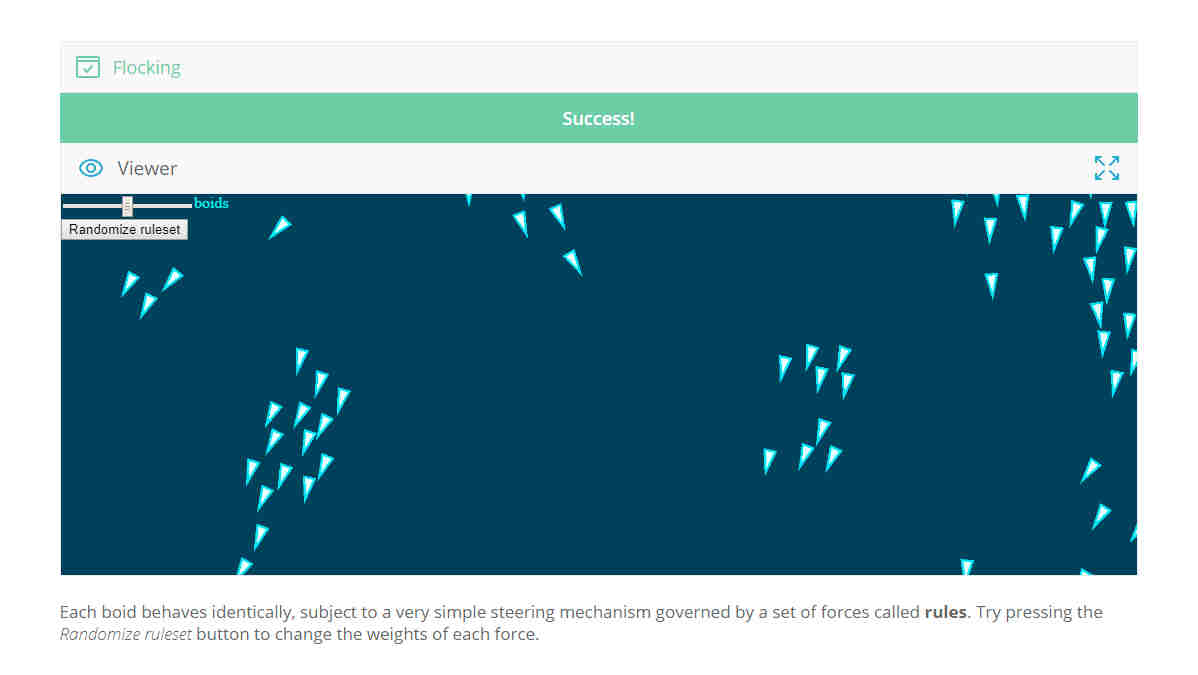
\includegraphics[width=\linewidth]{img/techio_game.jpg}
        \caption{A game developed and available in a \techio{} playground.}
    \end{subfigure}
    \hfill
    \begin{subfigure}{.45\linewidth}
        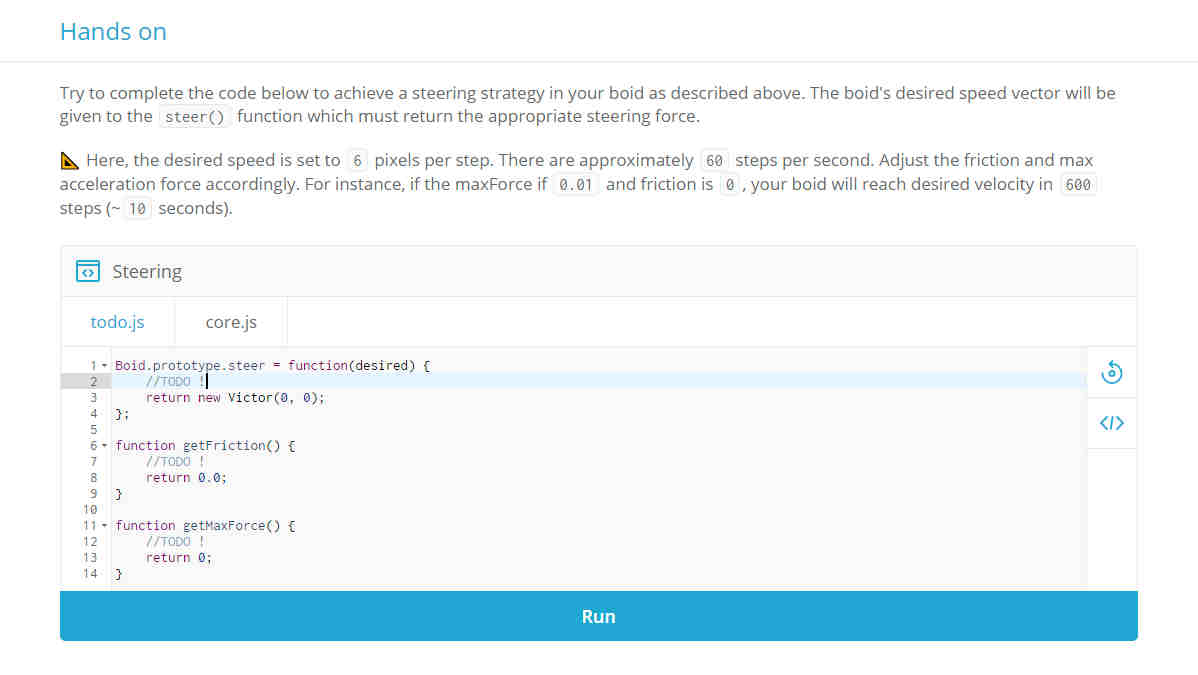
\includegraphics[width=\linewidth]{img/techio_handson.jpg}
        \caption{Coding in \techio.}
    \end{subfigure}
    \caption{Example pictures from \techio.}
\end{figure}

An investigation into alternative platforms to tech.io was launched. After some time of searching for a suitable alternative over the internet it was concluded that no platform really matched the requirements that were set. For the most part, only complete platforms with code verification were found that had closed APIs.

An example of such a platform would be code academy, which is an educational platform dedicated to providing the best learning experience for coding over the internet. However, it did not support individuals creating their own courses or using their code validation, hence it was not a viable candidate.
\begin{figure}[h]
   \centering
    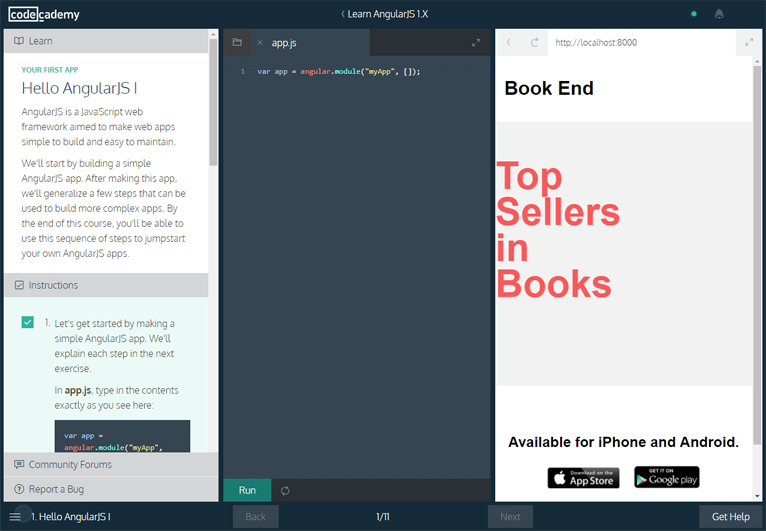
\includegraphics[width=.75\linewidth]{img/codeacademy_code.jpg}
    \caption{Example picture from codeacademy.}
\end{figure}


In contrast to \techio{}, a student at \LTU{} has developed an open platform called \sockr{} for hosting programming ladders. However, while the solution was more interesting from a licensing point of view, the source code of \sockr{} was mostly undocumented. It didn't have a clear API and the backend and frontend were too tightly coupled to be used in a sustainable way. It would require too much refactoring to be of use in the project.

After much research it was concluded that the best and most sustainable solution for the project would be to develop a code verification/compilation platform from scratch, effectively making the project completely independent of other services.


 \chapter{Design}

\section{Architecture}
To isolate the different parts of the system and limit overlap between groups, the project was divided in accordance with figure~\ref{fig:architecture} into three parts, frontend, backend and tester.

Frontend was designed to avoid keeping state. By doing so, the user-facing components could scale out to multiple backend servers and keep commonly used content cached. This would allow for better load-balancing where frontends could be geographically distributed and yield lower latencies.

Backend was designed to control the database and to keep a centralized management of state transitions. A feature that was discussed, but not investigated, was to shard the data between backends. That would have allowed even greater flexibility in the development of the platform, should it be used in more than one place.

Since tester could be used by other projects than the Gamified Programming Platform, it was designed to be idempotent and stand-alone. This meant that any tester server would yield the same result every time it was queried and have no prior knowledge of the system.
\begin{figure}
    \centering
    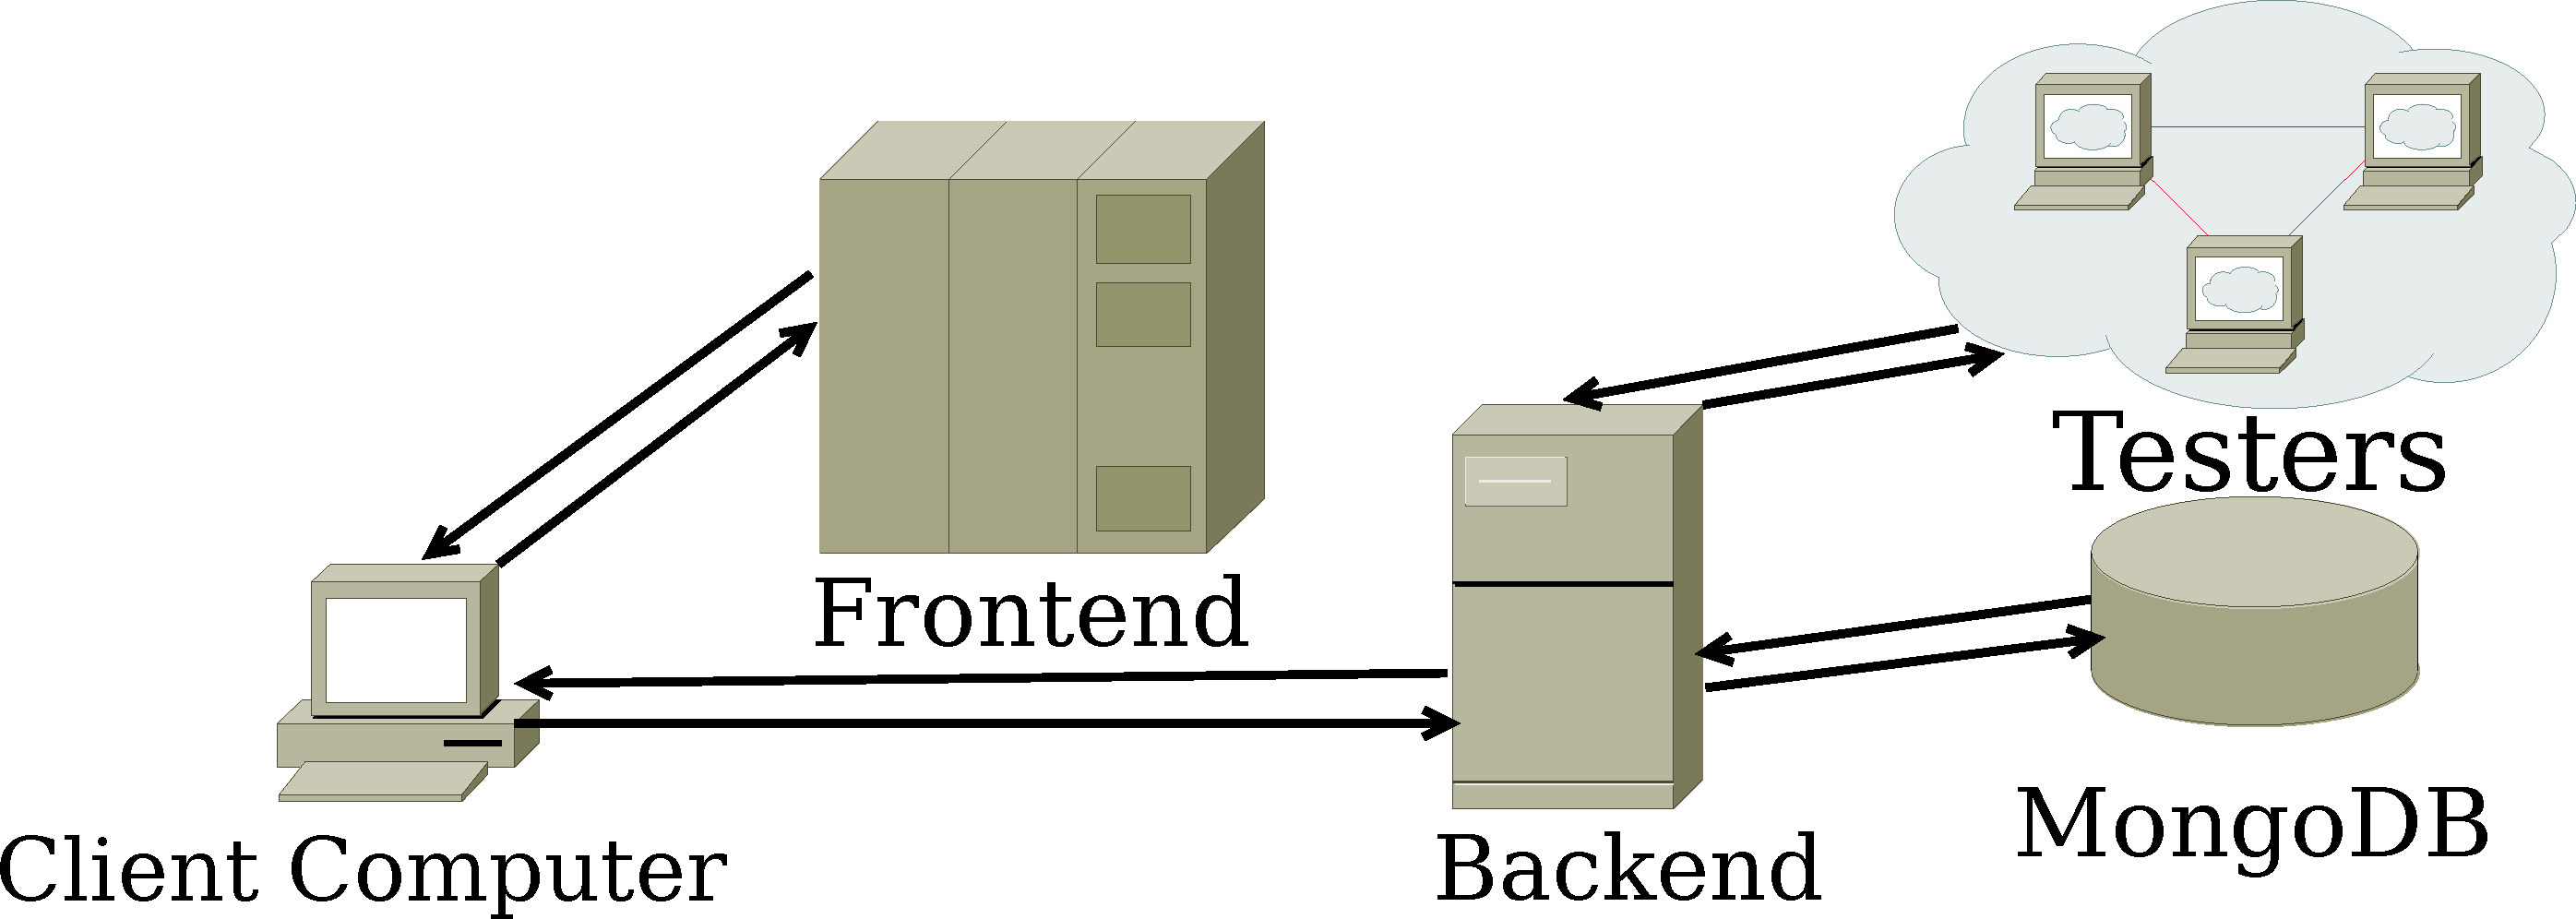
\includegraphics[width=.9\textwidth]{img/architecture.pdf}
    \caption{An overview of the architecture: First, some client interacts with the frontend, which uses javascript to send requests for resources on the backend. Then, the backend communicates with its database to serve resources. When the backend receives a request for testing, it retrieves assignment information, couples it with input data and sends it to the testers, which respond with the result of the test back through the request chain.}\label{fig:architecture}
\end{figure}


\section{Frontend}
\subsection{Authentication}
\subsubsection{Login}
To authenticate yourself on login you are by default prompted to sign in with LTU's weblogon CAS (central authentication service). 
This provides you with a ticket as an URL parameter and redirects you to path: $https://frontend\_ip/Auth$ which in turn contacts backend with said ticket to check its validity. If validated the backend responds with a status code of 200 OK and a JSON object containing authentication tokens for the user which are saved in local storage. In any other case the user receives status code 401 unauthorized and is prompted to login again.
\\
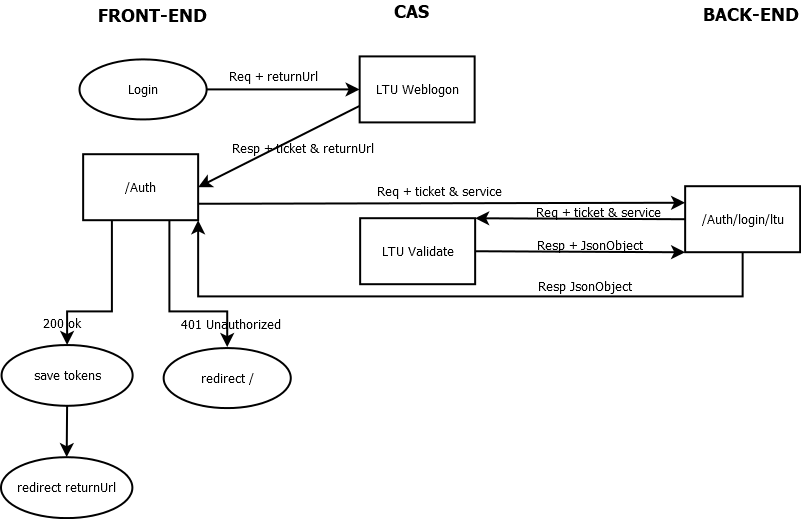
\includegraphics[width=\textwidth]{login.png}

\subsubsection{Auth interceptor}
The main purpose of this interceptor is to modify all requests by setting the authentication field in the header of the request for authenticated users. More than this it collects failed requests in the case of token expiration and tries to refresh the token to retry all failed requests automatically and stay logged in without the user being aware of affected.


\section{Backend}
% TODO move to a higher level (working methods?)
% A coding-standard was quickly decided on to make sure the code style was somewhat coherent effectively making it easier for different members to take over other members code if needed.

The backend of GPP was developed using javascript running with \nodejs{} as server framework and Express as a webframework to handle routing. \nodejs{} was chosen because it was the most established framework with wide support and multiple extensions, such as Express.

\subsection{Database} \label{database}

%OLD TEXT COMMENTED
%The document database MongoDB was chosen for the project instead of using a relational database, %the reasoning for this decision was to have a database that was built with scalability in mind %and dynamic schemas but also because of the simple reason that it is easy for the programmers to %read and understand the data inside the database thanks to MongoDBs JSON-like document %structure.
%OLD TEXT COMMENTED

MongoDB was chosen mainly to complete the MEAN software stack (MongoDB, Express, Angular, \nodejs{}). The majority of the group members working on backend did not have prior experience working with NoSQL databases which presented a good opportunity to learn. MongoDB is a popular choice among NoSQL databases and the group deemed it able to simplify when interacting with the data: Mongo uses a JSON-like document structure and JSON is the data format used when different parts of the project services communicates. 

Mongoose is a package that extends MongoDB by enforcing a database structure. With Mongoose it's possible to create schemas that describe the format of the data that is to be stored in the database. Mongoose presented a problem to the project members by not having consistency. If the schemas were updated there would be a mix of data, some of it stored in the previous format and some in the new. This resulted in a need to either migrate or remove the data in the database after schema updates.

While developing it also proved valuable to have a graphical representation of the data. The data is displayed using \href{https://github.com/mrvautin/adminMongo}{AdminMongo} which also enables the user to create new entries, edit existing data and delete data. Being able to insert and edit data presented some issues throughout the project since the user has full freedom when inserting data. No input validation or checks to the current database schemas are made. 


\subsection{API protocol}
A decision was made early in the project to adhere to a RESTful API design. Access paths to resources are built from the database schema~\ref{fig:schema}. For example: in the current database design, each assignment belongs to a course. It is therefore necessary to reference a specific course to access an assignment. Example: \texttt{GET https://.../api/courses/\allowbreak123123123/assignments/456456456/} returns assignment \texttt{456456456} which belongs to course \texttt{123123123}. Each resource name such as \texttt{courses} is in plural. A POST to \texttt{https://.../api/courses} creates a course while a GET request to the same resource returns all courses.

Data can be sent to the backend via both body and URL. Sending data via body is relevant for PUT and POST requests. The information for such requests should be sent as JSON and it should match the format specified in the API documentation~\ref{apidocs}. JSON is also the data-type used by the backend to return data, even when the result returned is a status code.

% errors
\subsubsection{Error handling}
To enhance a user's experience when working with the API, it was decided that a good way to handle both user errors and server errors should be implemented.

A server error is defined as an unexpected error that could cause the server to crash and therefore become unresponsive. A server error should never prevent the server from continuing serving data from working routes. Therefore every server error is handled and returned to the user as a HTTP error, 500 Internal server error. As explained in logger section(REFFA LOGGER SECTION) a server error is logged to help maintainers localize where things went wrong. This also prevents the server from crashing but the route which threw the error will still throw the error until it's patched. 

A user error is defined as any error caused by a user of the API. Trying to call a non existent route, not including input or including the wrong input are examples of user errors. If such an error is encountered it's important that the user receives feedback on what they are doing wrong. Both a fitting HTTP error code and error message should be returned. If a user has missed one required input field they should be told exactly which field is missing. All user errors is returned with a HTTP error code of 4xx.

Another type of user error occurs when the user makes a valid request which can not be handled because of restrictions implemented in the API. For example, if a user tries to modify data which they don't have access to. These errors is still considered user errors and will follow the error form of such an error.
% extensibility in features/progress/gamification

\subsection{Security}

\subsubsection{Authentication}
The API endpoint \url{/auth/login/ltu} validates a service ticket issued by CAS at \url{https://weblogon.ltu.se/cas/login} and, if successful, will issue an access token for use at the other access restricted endpoints of the API (see \ref{fig:auth}). The access token is a JSON Web Token with a short life span that is tamper proof and contains information about the user's id and access level. This approach allows the backend to remain sessionless, as the backend will validate the token at every API request. Since the access token expires quickly a refresh token is issued alongside it. The refresh token has a much longer life span and its only use is to generate new access tokens at the \url{/auth/login/accesstoken} endpoint. The refresh tokens are stored in the database, while the access tokens are not. Revoking a refresh token is done by deleting it from the database. Theft of an access token or refresh token would give the thief access until the token expires or, in the case of refresh tokens, it is revoked but this is made harder with SSL encryption.

\subsubsection{HTTPS} \label{https}
Self-signed certificates have been used for the testing environment in order to establish a secure environment with HTTPS. Once a proper production environment is used, it is preferable to use a trusted certificate authority instead of self-signed certificates.

\subsubsection{Input validation}
A common security problem in databases is injection attacks. To prevent this the API has to make sure the input has the expected form. A boolean input field must be of boolean type to be accepted. To achieve this, the module express-validator(REF https://github.com/ctavan/express-validator) was used. With this module it's possible to check URL, query and body input. For every invalid input field a specific error message is added to an array. When all fields have been checked, this array will be returned together with an HTTP error code 400 as feedback. This way the user can receive direct feedback without the need to consult the documentation. 

% SSL (HTTPS), just mention it
\subsubsection{Access control}
The API has three different base roles, 
\begin{itemize}
\item Basic
\item Advanced
\item Admin
\end{itemize}

These are assigned according to the user's role in their school, which is found when logging in through CAS. If the user is a student he will be assigned the basic role and if he is a teacher the advanced role is assigned. Admin is never assigned automatically and have to be set manually if needed. Depending on the role, different limitations are enforced. A basic user is only allowed to create 3 courses. Admins and advanced users are allowed to create an unlimited number of courses. This is the only difference between a basic and an advanced user. The reason a basic user is limited in their number of courses is simply to prevent malicious behaviour. Admins have full access to every route and are not limited in any way. This is mostly affecting course routes. 

Regardless of a user's base role he has a different role in every course. Every course in turn has three user roles,
\begin{itemize}
\item Student
\item Teacher
\item Owner
\end{itemize}
A student is only allowed to do things regarding himself, such as submitting assignments or leaving the course. The teacher role is to maintain the course but also to control who is allowed to join it. The highest course role is the owner which is the user that created the course. The owner can do everything a teacher is able to do, the only difference being that teachers can't remove the owner from the course. A user with the admin base role is basically able to do everything in any course.

\subsection{Quality control}
% jenkins
\subsubsection{Jenkins}
As a way to keep the project effective it was determined that it was important to implement continuous integration as a part of the project to have a modern workflow where you could push changes to git and have them automatically built on a live test server. Using continuous integration was also a good way to separate production and development builds and a way to ensure that production builds always kept a certain standard and robustness. The framework that was used for continuous integration was Jenkins which is one of the most popular frameworks.

While the idea of how continuous integration was supposed to be used in the project was quite clear, the concept wasn't put to as good use as it could have. In the first half of the project, the builds generated from Jenkins wasn't really put to use. This was mainly due to communication errors and the fact that the builds weren't needed as much. For the second part of the project the builds were used more. The way that the deployment with Jenkins was setup was to build from two branches from GIT, one from the master which was supposed to build for production and another from the backend branch which was supposed to build for development. The idea was that the development build would always contain the latest changes in backend. As the project reached its deadline it became increasingly important to also keep the backend dev builds stable because of the fact that the frontend team were depending on the backend dev build when developing.

Because of the increasing demands on having stable backend dev builds, a new requirement was setup for the continuous integration where a new development dev build was only built if it passed a set of unit-tests for the application.

% different environments
\subsubsection{Different environments}
Connected to the reasoning of building the backend in different environments/modes such as production or development, it was important to load different configurations depending on what environment the backend was supposed to run. For example, the production environment should not use the same database as the development environment. Because of this, it was important to be able to run the backend in different modes and dynamically load the correct configurations based on the mode that the backend was running in, hence a system that did this was implemented.

% logging
\subsubsection{Logging}
A large part of developers and support teams work is monitoring, debugging and troubleshooting. Because of this it is important to have good logging as a way to make these processes easier, faster and smoother. Having good logging gives them a good insight into what the application is doing and how it works. Because of this, it was important to have proper, useful and extensible logging available in the backend. A custom logging system promtly named logger was developed that ran with Winston and Morgan at its core. Winston is a simple and universal logging library and Morgan is a HTTP request logger middleware. Logger combined winston and morgan with the selectiveness of running the backend in different modes/environments. Depending on the mode, logger had different parts that it logged into log files.

Logger was setup to log all errors, server errors and a general logs in separate log files. When running in dev mode it was also important to log to the console, but not otherwise, hence console logging was only enabled when the backend ran in dev mode. 

Winston and Logger use levels to identify what type of information a log contains, the logging levels in logger conform closely to the severity ordering specified by RFC6424.
The severity of all levels are numerically ascending from most important to least important.

\begin{enumerate}
  \item Server Error
  \item Error
  \item Warning
  \item Info
  \item Verbose
  \item Debug
  \item Silly
\end{enumerate}

% automated testing
\subsubsection{Automated testing}
The API is a large part of the backend codebase. Automated tests of the endpoints were developed, mainly to guard against regressions. The tests mostly assert that the server doesn't return an error when given good input. In order to save time in test development, the tests are run in order, where older tests create the resources that are needed for later tests. This is not good practice in automated tests, but it would have been far more costly to make the tests independent of each other by doing setup and teardown for each endpoint test.


\section{Tester}
% intro, what is Tester trying to do?
% we want broad language support
Tester is a tool for testing code in a variety of programming languages in a safe and isolated environment. To fulfill the needs of the GPP, Tester needs to support a  broad variety of languages, so that the range of courses that can benefit from the platform is not limited. Tester also strives for the functionality to test code based on different merits to support the creation of varied, fun and interesting assignments.

\subsection{Sandboxing}
%TODO ref to docker
An important feature of Tester is that the code is tested in an isolated environment. The main reason behind doing this is that we are executing potentially malicious code. Allowing such code to be executed without isolation is bound to cause service disruptions or information leaks.

To achieve isolation all code testing takes place in so called Docker containers equipped with the tools necessary to compile and run the code. A container is a virtualization (simulation) of an operating-system with a separate user-space. What this means is that programs running inside the container can only access the contents and devices that are assigned to the container. By running the tests in Docker containers, any malicious code cannot gain access to information it shouldn't have access to or cause any disruptions to the service, since such code will at most crash the container which has no long-lasting effects on the service offered by Tester.
\subsection{Manager}
% add discussion of different ways of managing load and what we chose
% (Start containers on demand? Keep a pool of containers ready? Predict load or just react? Allocate different amounts of resources for different languages?)

As Backend sends requests to Tester these requests are handled by assigning a free container to serve that request.
If all containers for a language are busy, requests for that language are enqueued. 
The containers take around one second to start (NB:\@ on the authors' servers). In order to decrease the response time to backend,
containers are started preemptively. Once a request has been served another container of the same type is started.

If Tester receives a lot of requests, it will in turn start large number of containers.
Starting too many containers will affect the overall performance of the system and therefore performance per container.
This will increase the uncertainty of the timing tests which is undesirable.

In order to address this issue the Manager has to keep track of which containers
are started and which ones are currently processing a request. 
It is possible to configure the maximum number of containers that
can be started and to specify the maximum number of containers
per supported language. It is also possible to configure the number of containers
that should be started even if no request for that language has been made to keep
idling containers ready serve new requests. This is done in order to decrease
response time to Backend.

Each container is limited to one thread of the processor running at 50\% core speed and
100MB memory. Because of this each time a student runs the same code a similar
result can be observed. Timing is always a difficult property to measure but with
these settings Tester can deliver similar timings multiple times.

If a container is hijacked by malicious code the Manager has a timeout that will
force the container to exit and respond with an error.

\subsection{Test types}\label{sec:testtypes}
% unit tests are hard to write
% I/O tests are language-independent which is good if we want broad language support
Currently, Tester supports three types of tests:
\begin{itemize}
\item Input/Output (I/O). The submitted code is supplied with some input (either through standard in or commandline arguments) and the output is compared to what the code is expected to output.
\item Code size. These tests enforce a maximum limit on the number of characters there can be in the submitted code.
\item Lint. A lint test makes sure that the submitted code adheres to some coding standard for the language. Indentation, trailing whitespaces and blank lines are some examples of what might be checked.
\end{itemize}
When deciding which test types had the highest implementation priority, an important factor was the time expenditure required by the creator of the tests. If writing tests for a single assignment takes a considerable amount of time the platform will become impractical to use. For this reason tests such as Unit Tests are not supported. It would be time-consuming for lab supervisors to write tests.

Another deciding factor is the language-dependency of the unit tests. If a test requires language-specific implementation the extensibility of the language support suffers. This is one of the reasons why the I/O and Code size tests mentioned allow are excellent choices, they are both language-independent and require no additional implementation for every language supported. Although Lint tests are not language-independent, they have been implemented for a few languages as a proof of concept.

\subsection{Extensibility}
In order to achieve broad language support, it needs to be easy to add new languages. Two steps are necessary to add support for a new language:

\begin{itemize}
\item The manager has a makefile that produces docker images for each supported language. The makefile needs to be extended with a new target that installs language-specific dependencies.

\item The Node instance running in the container needs to have a module for each supported language. Each language module exports two functions: \texttt{prepare}, which produces a file that can be run with the \texttt{run} function. The \texttt{prepare} step is used for compiled languages, where a binary must be produced before running the program. Some languages, such as python, are run directly in the interpreter. By making preparation a separate step, the program does not need to be recompiled for each test.
\end{itemize}

\subsection{Service Availability Fallback}
A little known feature of Tester is that it plays nice with load-balancers by reporting whether or not the testing service itself is available. That is, if the language that is to be tested isn't available, or the testing-queue is full, it defers the job to another Tester. It does that by responding with the \texttt{503: Service Unavailable} status, after which the load-balancer sitting in front of it will understand that it needs to route traffic elsewhere.


 \section{Working methods}
\subsection{Sprints} 
Agile work flow was used during the project. This was done by dividing the weeks into sprints. A sprint was expected to be one week but sometimes sprints become longer due to heavy workload. Every sprint was planed before the current sprint was ended. The group leaders planned the sprints, one from each current sub group along with the project leader. Taiga.io, a sprint planning tool kept track of the backlog and different task assigned to individual group members. This showed which task was completed and which needed to be helped with. During the project some of the members evaluated the tool Taiga.io and found that it could have been better if it was possible to add tasks to more than one person, if it was easier to assign points to a task and move a task to other sprints. A decision was made to keep Taiga.io because the members had gained experience with it and it would be impractical to split the backlog to a new tool.

\subsection{Groups} 
All of the different task sections were split into groups. During the project it was laborated on how many number of groups would be the most efficient for the project. The working model that was found was to have three groups with 4-5 members each as long as there were enough tasks in different sections for three groups. Every week at least one time all members met and discussed the previous week and the upcoming week. This became a meeting with 15 people that ended up talking over each other which felt ineffective. This was solved by minimizing the meeting members to three-four people: the project leader along with one group leader each from the frontend, backend and tester group. The leaders were democratically chosen in each active group and their task was to tell the other group leaders what they have and will accomplish during next period. They then went to their own groups and told them about the meeting. This worked well during the first weeks but less and less information were distributed to the group member as time went by. When this problem was then identified it was to short time left on the project to change the meeting method and instead it was simply decided that everyone needed to try and keep the quality of the distributed information up like it was in the first few weeks. \\
The different groups that has been presented are:\\
 \begin{itemize}
 \item Interviews
 \item Workshop
 \item Platform
 \item Theory
 \item Frontend
 \item Backend
 \item Tester.
 \end{itemize}


\subsection{Roles} 
All the project members had a responsibility that the project should succeed and it was important to contribute to the extent that each member was capable of.\\
The three major roles have been assigned during the project, these are \\
\textbf{Project leader} - Niklas Fuks which had an overview of the project and its sub tasks. Planned the meetings, sprints and held presentations with demos. \\
\textbf{Groupleader and software engineers} -\\
Axel Sundbom (tester)\\
Tobias Axelsson (backend) \\
Axel Vallin (frontend) \\
\textbf{Software engineers} -\\
Linn Danielsson\\
Nils Fitinghoff\\
Mikael Hedkvist\\
David Sandström\\
Anton Jerhamre\\
Christopher Rosenvall\\
Fredrik Bostrand\\
Henrik Nilsson Harnet\\
Tim Granström\\
Rickard Nordlander\\
Anders Mikkelä\\

 % TODO: this should be place somewhere more appropriate
\chapter{Workshop}
\label{sec:workshop}
As a part of the prestudy, educators and a few students were invited to a platform-development workshop. During the event, participants were divided into groups and asked to develop their own mockups for educational services according to the script below.

\section*{Introduction (10min)}
We are studying the fifth year at computer science program at LTU and for now doing our project. As a part of our prestudy are we hosting this workshop where we will investigate possibilities through a couple of scenarios. You will do a couple of assignments in groups and then present your result and discuss these with others.

\section*{Scenario 1 (10 min + 10 min discussion)}
You have just started a course in which you will learn to program in a language that you don't find interesting. The teacher has given you a lot of recommended exercises but they don't seem very interesting. Which type of system or moments would motivate you to do the assignments. Associate freely.
\begin{itemize}
\item Which subject do you think has this problem?
\item Do the assignments need to be presented? If so, how?
\item Which material is needed?
\item If you were to make a list of highlights, what would be on it?
\end{itemize} 

\section*{Scenario 2 (10 min + 10 min discussion)}
After many years, you find yourself teaching that boring course. The boss comes in to your office late one Friday afternoon and says that the course moments are too few and that you need to update them before Monday. You sit down as the motivated teacher you are and contemplate what kind of system that would motivate students. Suddenly, you remember your old concept.

You want to make this work in the long run, which limitations must you as a teacher do?
\begin{itemize}
\item What is most time consuming?
\item Is it possible to sort your highlights by time required?
\item How many hours would be required to develop and maintain the solution over time?
\end{itemize} 

\section*{Scenario 3 15 min + 10 min discussion}
Now your system works well for that boring course and with a little tweaking, it should work with all those new courses you'll be giving. However, it is 2017 after all and the students are crying for a web-based tool. What does this tool look like? Model a web-page to fit your tool.

\begin{itemize}
\item How do you handle inputs?
\item What do your highlights look like in practice?
\item Do you see any limitations?
\end{itemize} 


\section*{Results}
A set of project proposals for a web-development course was written as a result of the workshop, these proposals can be found at \url{https://github.com/ax-rwnd/m7011e-projects}. Furthermore, a list of ideas and reflections noted in the workshop

\subsection*{Scenario 1}
\begin{itemize}
\item Let assignments interlink.
\item Be able to choose which assignments should be done.
    \begin{itemize}
    \item Hard to grade, every goal of the course need to be met.
    \item Assignments with similar content.
    \end{itemize}
\item Constructive alignment, how goals, assignments and examination interacts.
\item Early and quick feedback.
\item Formative assessment, continuous feedback.
\item Group assignments, hide the personal result.
\item AI Avatar that gives feedback.
\item Lot of visualization of the result.
\item Present the purpose of the assignment.
\item Different angle of the design depending on the user which is solving the assignment.
\end{itemize}

\subsection*{Scenario 2}
\begin{itemize}
\item Not everything in a course should be changed at the same time.
\begin{itemize}
\item Old assignments could be divided.
\item Shorter feedback loop.
\item Old assignments with new context.
\end{itemize}
\item Updating the course introduction is cheap and makes the goals of the course more clear when the knowledge is to be tested.
\begin{itemize}
\item Thoroughly, min/max, median or average.
\item In the end there is a written exam.
\end{itemize}
\item Retain results from previous students
\begin{itemize}
\item Keep old posts in forums.
\end{itemize}
\item Peer-to-peer feedback.
\item Test an implementation even if it's bad to receive feedback.
\item Students create assignments for each other.
\end{itemize}

\newpage
\subsection*{Scenario 3}
\begin{itemize}
\item Anonymous questions
\begin{itemize}
\item ``Did you understand what I said?''
\item Direct feedback.
\end{itemize}
\item Direct chat between students and teacher.
\item Auto generated feedback to the teacher.
\begin{itemize}
\item Aggregate data from relevant measurements.
\end{itemize}
\item A student knowledge bank.
\begin{itemize}
\item Wiki format.
\end{itemize}
\item Code correction / evaluation.
\end{itemize}

\vfill
\subsection*{Photos}
\begin{figure}[hb]
\centering
    \begin{subfigure}{.32\textwidth}
        \centering
        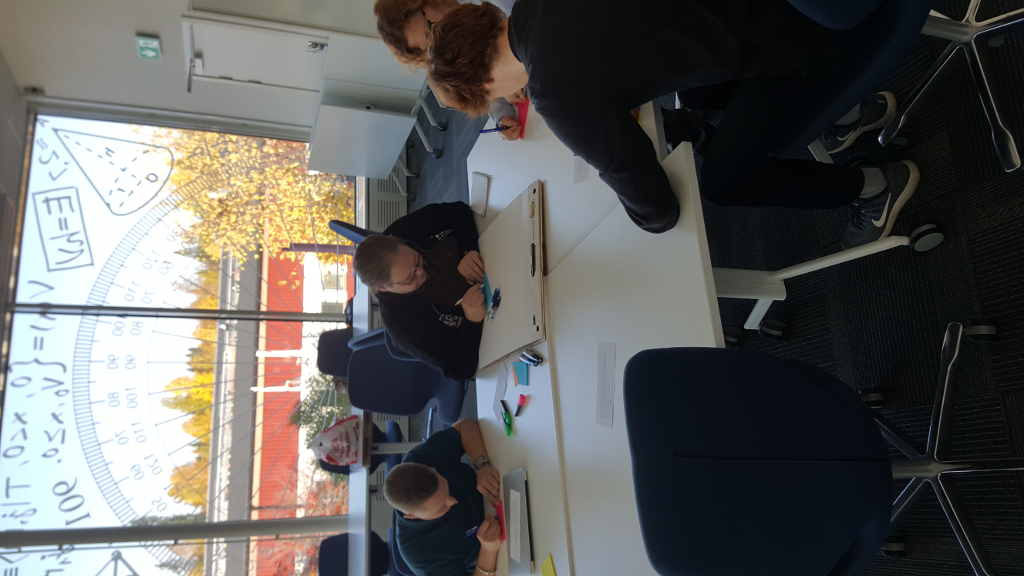
\includegraphics[width=\textwidth, angle=270, origin=c]{img/workshop1_resized.jpg}
        \label{fig:workshop1}
    \end{subfigure}
    \begin{subfigure}{.32\textwidth}
        \centering
        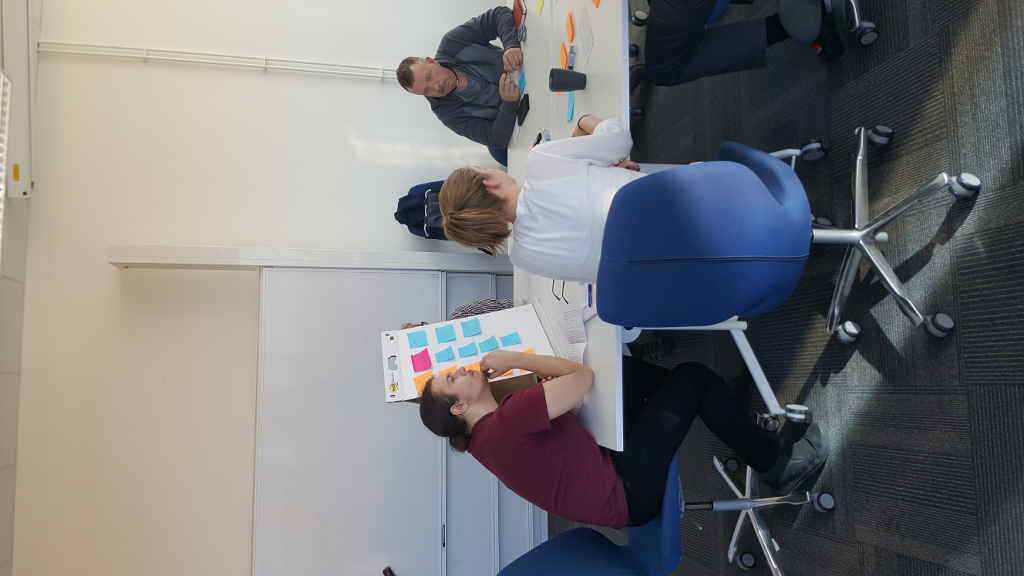
\includegraphics[width=\textwidth, angle=270, origin=c]{img/workshop2_resized.jpg}
        \label{fig:workshop2}
    \end{subfigure}
    \begin{subfigure}{.32\textwidth}
        \centering
        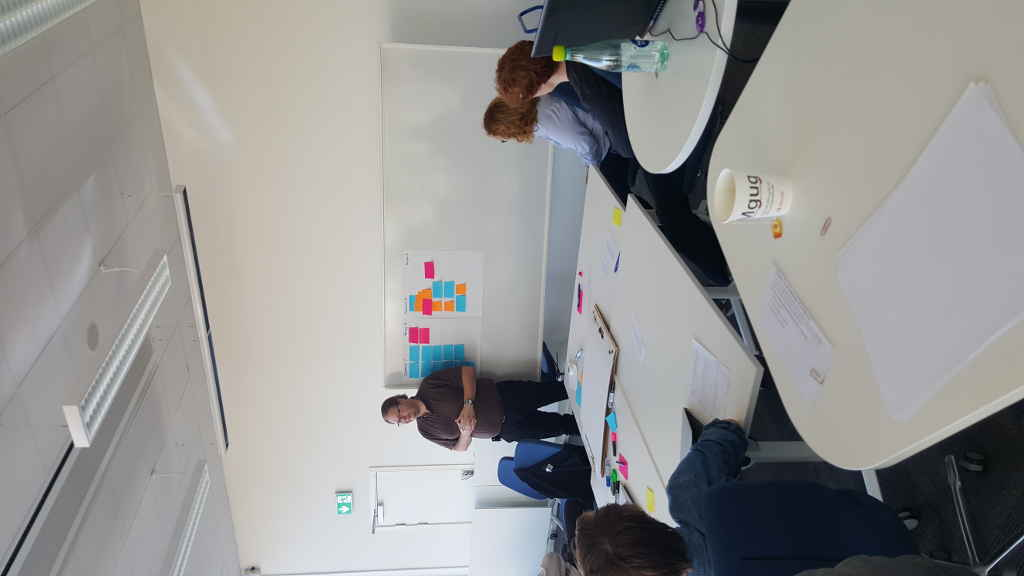
\includegraphics[width=\textwidth, angle=270, origin=c]{img/workshop3_resized.jpg}
        \label{fig:workshop3}
    \end{subfigure}
    \caption{Workshop}
\end{figure}
\vfill


 \chapter{Discussion}

\section{Evaluation}
Initially, we set out to build a system that would make learning programming more fun and less tedious. This would involve gamification as a mean of picking up weaker students that would otherwise fail and give up in the face of overwhelming challenges. In addition, we wanted to remove, or at least lessen, the requirement of having personnel hired to correct labs by using automated correction.

To solve the automation, a system was developed that would create sandboxes, perform simpler tests and allow easy extensions. This way, other maintainers could add their languages of choice to the solution at a later time and select which testers they would like to use based on what languages are available and what latency they provide. Furthermore, this system was designed to scale out horizontally, meaning that if the system needs to be used by a larger amount of people, more hardware can be added to match the increased load.

Something that was not planned, but came as a consequence of how the tester was developed, is that the tester is so generic that it can be used for other projects as well. This opens possibilities for authors of similar services and games to develop new frontends quickly that make use of the service instead of reinventing it.

On the other hand, an issue that teachers of more advanced courses may have with the system is the lack of real unit tests. Without unit tests, making conclusions about application internals is nearly impossible and requires student interaction. However, an attempt was made at implementing unit testing for \emph{any} language, which showed that it could be done, see section~\ref{sec:testtypes} and section~\ref{sec:unittests_future}, but was eventually thrown away as the implementation proved both messy and hard to set up for teachers.

For the other part of helping students discover the joy of programming, like we already have, we have built a website that is both a game and a learning platform. While the game itself is not the most exciting piece of work to see the light of day, it does not spoil students into requiring games to learn either. By keeping the process of creating new game elements simple, we hope that it will be possible for others to create new elements on their own. This includes the ability to create elements that do spoil users and other bad things, but that will need to be formally evaluated at some point.

The provided modules showcase some simpler mechanics that can be woven into the service and that expose both positive and negative traits. For instance, the progress bar \emph{may have} the negative effect of not promoting learning beyond the platform, but to prove that it does, empirical data must be gathered both from the platform and from real life. Our system lets educators and researchers gather this data by running courses with and without game elements included. This data may then be compared to the success/drop-out-rate of the students attending the course.

Unfortunately, an important mechanic that we had hoped to implement, but were unable to realize in time, was group effort. A common theme discovered in the prestudy was that letting students cooperate and interact with other students introduces some interesting boons. Some angles that could be explored are further documented in section~\ref{sec:social}, but were considered too big of a risk to actually commit to at the late stage of development when the single-player elements were finished, as it might carry the hidden requirement of editing the database schema.

Fittingly, this brings us to the issue of maintainability and extensibility in the database. It was discovered, when introducing the game elements, that the database structure that had been developed could not support the level of modularity we wanted to offer. As an effect, storing custom data for game elements may require both API modifications and updates to the database schema. For the amount of game elements included in our release, it serves fine, but in extension it might not scale.

In conclusion, the service is able to provide a fun and engaging experience for students that does not necessarily spoil them into not studying. Meanwhile, educators are able to create courses that allow students to complete assignments and get rewards appropriately. This is done in a manner that can partially replace lab assignments and retain more students, all the while saving working hours that would otherwise be spent on correcting labs. Lastly, new game elements can be created by educators and researchers alike to expose data that is critical to research within the field of gamification within education.

% TODO: connect with future work and A/B testing Even without A/B testing in the system, simpler statistical measurements should % TODO: mmention that not all elements are good% Also, with the modular approach taken to the game elements, new games can be created without too much work.





\section{Workflow}
There were 15 students in a project that was originally dimensioned for 7--9 students. Apart from the common issues that arise when managing very large groups, the oversized project group made members who aren't as used to voicing their opinions express themselves even less. This characteristic is also something that was discussed in the conducted interviews and the solution is usually to either help people trust one another (teambuilding), or to remove the requirement of trust (anonymization). 

The project specification didn't specify all details regarding the requested product. This lead to a long prestudy wherein a lot of time was devoted to answering questions that maybe could have been partially answered by the project owner if asked more thoroughly. No technical work was initiated before the prestudy was done, primarily out of the fear of performing work that would be thrown away if the project goal changed. In effect, a lot of people did very little work during the four first weeks. In hindsight a part of the group could have started looking into other technical parts that would be needed regardless of the results acquired in the prestudy.

Delegating all inter-group communication to the leaders was a challenge, probably because the needs were far too large. Most of the communication between groups happened in the project-room between developers. Another consequence of this is that developers that did not work from the project-room had trouble staying updated on the latest decisions and reporting their progress. This made it difficult to keep the developers saturated with tasks. The main problem was that information was spread in a non-standardized way which resulted in some people not receiving enough information. Taiga was initially used to delegate work and issues between members but over time it became less used and a classic whiteboard became the main source of delegating tasks. Based on the experience aquired from the project, it would have been better to decide on a communication method, stick to it and enforce it as a way to minimize communication errors.

The project leader, who should have an overview of the development, got information about the progress from the group leaders. This information was superficial and unable to compensate for the lack of communication with the developers. This lead to a lack of technical depth in the biweekly presentations. To increase the technical content of the presentations, the group leaders had to become more involved in them. The project leader should have been more present in the project room when the developers were there to gather information about the development progress. In conclusion, having too many levels of leadership did not work well for an organization of this size.

Structuring a functional workflow with 15 members was a big challenge and an invaluable experience for all members since no one had any previous experience in working with such a large group. Even though the group faced several issues and challenges, a product was developed that each and every one could be proud to have been part of.

subsection{Project Planning}
The agile development style was well-suited to the biweekly presentations. However, the group was not completely satisfied with \taiga{} as a sprint planning tool. There were many features that were not used because they seemed to only increase the burden on the developers. The group leaders found that transitioning between sprints required a lot of manual work. Partly as a result of the problems with the tool, tasks gradually transitioned to being tracked on a whiteboard in the project-room. This lead to a clearer picture of the current tasks for on-site developers, but compounded the previously mentioned problems for remote developers.


\section{End-Product}
We set out to build a website that could help examiners improve their courses by using gamification. To do this, both student interaction and teacher management had to be considered to create a pleasant user-experience.

Most notably, we aimed to minimize the unnecessary feedback loop between students and lab-supervisors. By creating an extensible and scalable tool for automated testing of code, we could provide an environment that our platform---and other platforms---can use to test assignments.

By implementing a framework that would allow quick implementations of new elements, a platform for researching new gamification tools was born. After implementing a new element, it can be evaluated by looking at the completion statistics. However, there is much work that can be done on this part to empower teachers and gamification researchers with the data they need to make conclusions regarding their original research.

As a deployment note, the solution should be fairly easy to install for the IT department. Our plan of action for doing this was to deploy frontend and backend as docker containers together with a haproxy docker container for load-balancing. Configuring these would be done using configuration files which the person deploying the solution could modify before building the docker containers, and thus set the correct settings for their setup. However, the tester environment requires docker to run, and should probably not be nested\cite{nesteddocker}, so that needs to run on its own virtual machine. Some additional work may be needed for the first deployment to generate a working configuration.


%\section{Conclusions}
%Gamification has become a large part of motivation. By getting rewards for performed works the motivation and satisfaction increases. Gamification with immediate feedback in programming is fairly new since learning programming has grown and spread to lower ages, a tool for learning programming quickly is needed.  
The platform provided is dynamic in that way that there is no limitation in the difficulty in the assignments, the creator of the assignment is that one which sets the level. By that said, even since the target is university students, the platform is also applicable to younger students. There are endless choices for new gamification parts that can be implemented, only the imagination puts a stop to which parts can be implemented. The platform delivered is an initial working product that is usable but can be expanded to fairly low cost. 


 \chapter{Future Work}

\section{File Upload}
A feature that is not currently supported is the option for users to upload files to the platform. This limits the teachers' abilities to upload backgrounds for the map and requires all students to write their code using the site's in-browser editor. The Ace-editor we are currently using is limited both in terms of features and customizability. Further, this would allow the student to write and save their code offline in the case that either the site is down or if they are in a location with no network connection.

Implementing this feature could require support on both the frontend and backend. If the file is stored as a file in the database, support for storing files would be required. But the code could also be stored as a string similar to how code submissions through the in-browser editor are stored, which would only require some parsing on the frontend side.


\section{Statistics}
As of right now, there is a simple statistics page that is implemented on the frontend for showing statistics for a specific course. A teacher can see pie-charts for each assignment in the course and how many students that has completed that assignment of the ones who are registered to the course.

The current implementation is using the API call to get all features for that specific course. This API call returns a lot of data that is unnecessary, and in some cases might not be correct to send to frontend. The data used for statistics has to be individually picked out from the massive response that the API call returns. In the future, it might be good to create a route from backend that returns the amount of students that has passed a specific assignment.

In the future, it might be nice to add a graph like the one in figure~\ref{fig:progovertime} for each assignment plotting when students pass a specific assignment. This feature would require the database to keep track of which dates students first pass specific assignments.
\begin{figure}[hb]
    \centering
    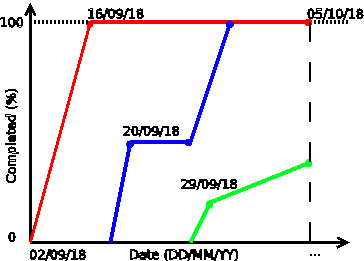
\includegraphics[width=.6\linewidth]{img_src/progress_over_time.png}
    \caption{What a time-progress graph could look like. Here, each color represents an assignment, but it could also be split into individual graphs.}\label{fig:progovertime}
\end{figure}


\section{A/B Testing}
A/B testing can be applied in various ways to measure how effective improvements and updates are to a service. This essentially means utilizing 2 different groups of users to discover behavioural patterns and interpreting the result from the difference in performance. In GPP this might be used to improve the user interface by finding better color combinations and/or element positions. More importantly, tests could be run by teachers and researchers to determine which elements work and which don't.

One way of implementing this in GPP could be to divide a fraction of the user base into groups, expose them to changes and monitor its effects. For instance, testing the adventure map might show a significant increase in performance for group A whilst group B shows no change. Furthermore, change could possibly be seen in the second group---despite there being no change to the group itself---as the total amount of completed assignments increases in both groups.

Given that enough users participate in the A/B study, it can be shown with statistical significance that a gamification element is either profitable or inconvenient. In extension, this allows examiners to convince their faculties by showing them data proving its usefulness, allowing them to implement it into their courses.

The reason for this not yet being implemented is primarily that it requires the correct statistics to be available for extraction. Unfortunately, little work was devoted into statistics aggregation on the backend, meaning that until recently, implementing statistics-based features was very cumbersome. With a further developed statistics feature, implementing A/B testing should be feasible.

\subsubsection{A Twist}
\begin{wrapfigure}[14]{r}{6cm}
    \centering
    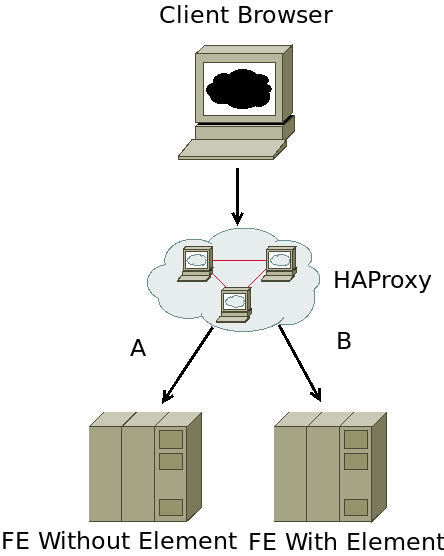
\includegraphics[width=.6\linewidth]{ab-loadbalanced.png}
    \caption{An alternative approach to A/B testing using the load-balancer.}
\end{wrapfigure}
Depending on what kind of statistics the A/B tests should determine, an alternative, more general approach could be taken. This works by implementing the testing \textit{on top of} the solution, instead of within, and may be easier to get started with. The drawback is that all tests would be done on a more coarse granularity.

Rudy Lee provides an example\cite{rudylee} for how this can be setup using the recommended HAProxy load-balancer. By first letting a balancing algorithm (round-robin, random or minimal-load) send users to a specific site and then setting a cookie to track and direct users on repeated visits, statistics like retention rate can be determined when doing site-wide changes. Unlike an A/B tester implemented inside the platform, this tool cannot capture changes done to single courses, only global ones, which limits the usefulness to educators.


\section{Extended Login Functionality}
Having more ways of logging in to the system, eg. \github{} or \facebook{}, would allow a greater number of people to access and try out our system. More users would also require finding a solution for scaling up the infrastructure to handle higher traffic.


\section{Predicting demand in Tester manager}
The way that the manager for Tester starts more containers for popular languages could be improved. The current solution indirectly bases the number of containers allocated to each language on the recent demand for that language. Instead of just adapting to load, the manager could use a model that predicts future load. This model could use more information than just the languages used in recent requests, such as which courses are currently given.


 \printbibliography{}
  \appendix

\chapter{Workshop}
% TODO: this should be place somewhere more appropriate
\chapter{Workshop}
\label{sec:workshop}
As a part of the prestudy, educators and a few students were invited to a platform-development workshop. During the event, participants were divided into groups and asked to develop their own mockups for educational services according to the script below.

\section*{Introduction (10min)}
We are studying the fifth year at computer science program at LTU and for now doing our project. As a part of our prestudy are we hosting this workshop where we will investigate possibilities through a couple of scenarios. You will do a couple of assignments in groups and then present your result and discuss these with others.

\section*{Scenario 1 (10 min + 10 min discussion)}
You have just started a course in which you will learn to program in a language that you don't find interesting. The teacher has given you a lot of recommended exercises but they don't seem very interesting. Which type of system or moments would motivate you to do the assignments. Associate freely.
\begin{itemize}
\item Which subject do you think has this problem?
\item Do the assignments need to be presented? If so, how?
\item Which material is needed?
\item If you were to make a list of highlights, what would be on it?
\end{itemize} 

\section*{Scenario 2 (10 min + 10 min discussion)}
After many years, you find yourself teaching that boring course. The boss comes in to your office late one Friday afternoon and says that the course moments are too few and that you need to update them before Monday. You sit down as the motivated teacher you are and contemplate what kind of system that would motivate students. Suddenly, you remember your old concept.

You want to make this work in the long run, which limitations must you as a teacher do?
\begin{itemize}
\item What is most time consuming?
\item Is it possible to sort your highlights by time required?
\item How many hours would be required to develop and maintain the solution over time?
\end{itemize} 

\section*{Scenario 3 15 min + 10 min discussion}
Now your system works well for that boring course and with a little tweaking, it should work with all those new courses you'll be giving. However, it is 2017 after all and the students are crying for a web-based tool. What does this tool look like? Model a web-page to fit your tool.

\begin{itemize}
\item How do you handle inputs?
\item What do your highlights look like in practice?
\item Do you see any limitations?
\end{itemize} 


\section*{Results}
A set of project proposals for a web-development course was written as a result of the workshop, these proposals can be found at \url{https://github.com/ax-rwnd/m7011e-projects}. Furthermore, a list of ideas and reflections noted in the workshop

\subsection*{Scenario 1}
\begin{itemize}
\item Let assignments interlink.
\item Be able to choose which assignments should be done.
    \begin{itemize}
    \item Hard to grade, every goal of the course need to be met.
    \item Assignments with similar content.
    \end{itemize}
\item Constructive alignment, how goals, assignments and examination interacts.
\item Early and quick feedback.
\item Formative assessment, continuous feedback.
\item Group assignments, hide the personal result.
\item AI Avatar that gives feedback.
\item Lot of visualization of the result.
\item Present the purpose of the assignment.
\item Different angle of the design depending on the user which is solving the assignment.
\end{itemize}

\subsection*{Scenario 2}
\begin{itemize}
\item Not everything in a course should be changed at the same time.
\begin{itemize}
\item Old assignments could be divided.
\item Shorter feedback loop.
\item Old assignments with new context.
\end{itemize}
\item Updating the course introduction is cheap and makes the goals of the course more clear when the knowledge is to be tested.
\begin{itemize}
\item Thoroughly, min/max, median or average.
\item In the end there is a written exam.
\end{itemize}
\item Retain results from previous students
\begin{itemize}
\item Keep old posts in forums.
\end{itemize}
\item Peer-to-peer feedback.
\item Test an implementation even if it's bad to receive feedback.
\item Students create assignments for each other.
\end{itemize}

\newpage
\subsection*{Scenario 3}
\begin{itemize}
\item Anonymous questions
\begin{itemize}
\item ``Did you understand what I said?''
\item Direct feedback.
\end{itemize}
\item Direct chat between students and teacher.
\item Auto generated feedback to the teacher.
\begin{itemize}
\item Aggregate data from relevant measurements.
\end{itemize}
\item A student knowledge bank.
\begin{itemize}
\item Wiki format.
\end{itemize}
\item Code correction / evaluation.
\end{itemize}

\vfill
\subsection*{Photos}
\begin{figure}[hb]
\centering
    \begin{subfigure}{.32\textwidth}
        \centering
        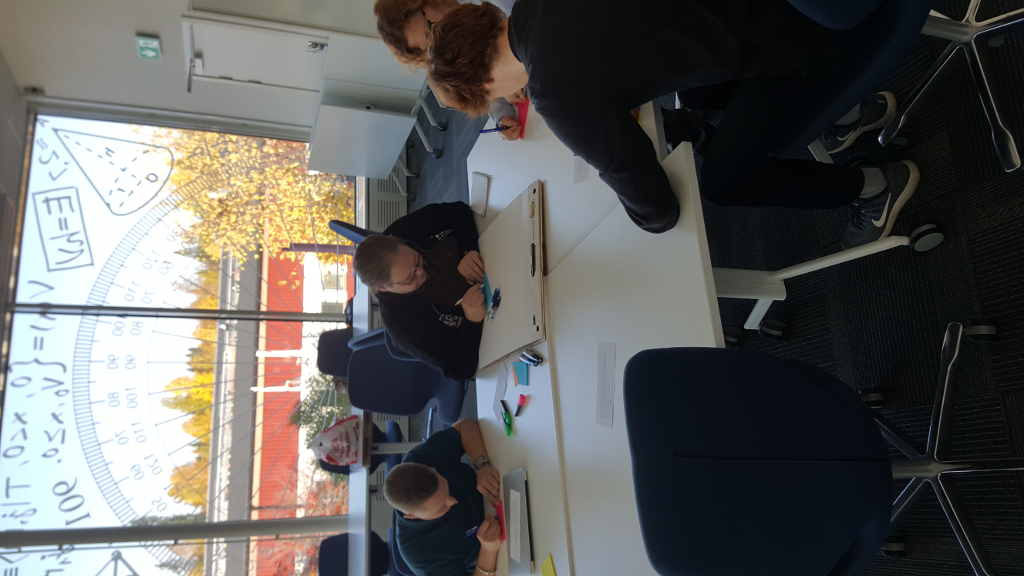
\includegraphics[width=\textwidth, angle=270, origin=c]{img/workshop1_resized.jpg}
        \label{fig:workshop1}
    \end{subfigure}
    \begin{subfigure}{.32\textwidth}
        \centering
        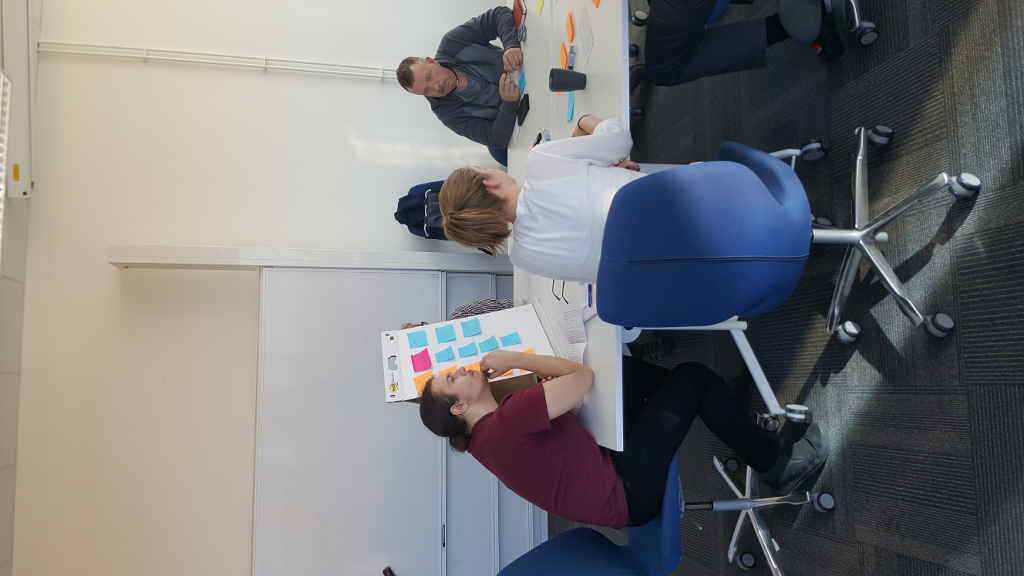
\includegraphics[width=\textwidth, angle=270, origin=c]{img/workshop2_resized.jpg}
        \label{fig:workshop2}
    \end{subfigure}
    \begin{subfigure}{.32\textwidth}
        \centering
        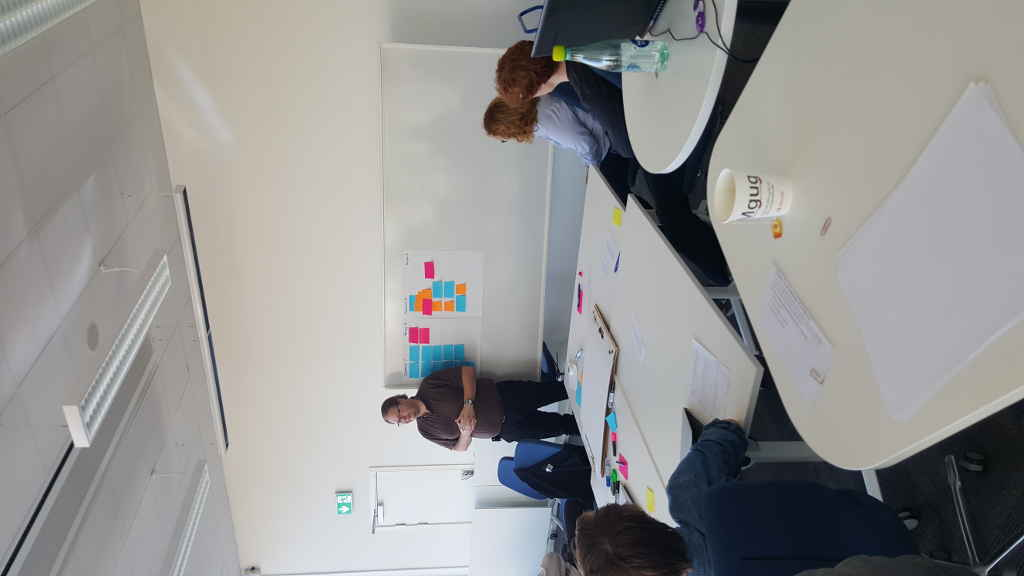
\includegraphics[width=\textwidth, angle=270, origin=c]{img/workshop3_resized.jpg}
        \label{fig:workshop3}
    \end{subfigure}
    \caption{Workshop}
\end{figure}
\vfill



\chapter{Installation Instruction}
The Gamified Programming Platform was a service was built and tested on debian linux 9 (stretch) with node 8.6.0 and npm 5.3.0.

\section{Tester}
Tester consists of two components; Manager and Runner. Managaer replies to requests from the backend and manages docker containers that run arbitrary code. Containers are used to ensure that some test A does not interfere with some later test B by modifying the executing environment.\\
\begin{enumerate}
    \item Clone the repo: \texttt{git clone \url{https://github.com/ax-rwnd/d7017e-project}}
    \item Change directory to the Manager folder: \texttt{cd d7017e-project/tester}
    \item Install the dependencies for the Manager: \texttt{npm i}
    \item (Optional) Select languages by adding/removing dependencies in \texttt{Makefile}. For instance the line \texttt{all: python27 python3 java c \# haskell} selects the languages Python 2.7, Python 3, Java, C, but not Haskell (since it's commented out).
    \item Run the Makefile: \texttt{make}
    \item (Optional) Set preferences for Runner in \texttt{config/default.js}. There, things like queue lengths and ports may be configured.
    \item Move back up to manager: \texttt{cd ..}
    \item Start Manager: \texttt{node server.js \{PORT\}}
\end{enumerate}

\section{Backend}
Backend is the state-managing component. It uses MongoDB to store information that it receives while processesing frontend requests and tester results.
\begin{enumerate}
\item Install och configure MongoDB.
\item Clone the repo: \texttt{git clone \url{https://github.com/ax-rwnd/d7017e-project}}
\item Change directory to backend: \texttt{cd d7017e-project/Backend}
\item Install dependencies: \texttt{npm i}
\item Configure database address/port in \texttt{Backend/config/default} and \\
\texttt{Backend/config/production}. IP/Port may differ between the files, should you want to use different databases for testing and production. To select one of these files, set the \texttt{NODE\_ENV} environment variable to \texttt{production} or \texttt{development}.
\item Start the backend daemon: \texttt{npm start}.
\item (Optional) Start start backend in the foreground: \texttt{node ./bin/www}
\end{enumerate}

\section{Frontend}
Frontend is the part that the users see. It builds on Angular for UI and contacts backend for functionality.

\begin{enumerate}
    \item Clone the repo: \texttt{git clone \url{https://github.com/ax-rwnd/d7017e-project}}
    \item Change directory to frontend: \texttt{cd d7017e-project/frontend}
    \item Redirect frontend to backend: \texttt{sed -i "s/ \textbackslash (backend\_ip: \textbackslash )'.*'/ \\ \textbackslash 1'\url{https://{your\_backend}}'/" src/environments/environment.prod.ts}
    \item Tell were the global ip for frontend is: \texttt{ed -i "s/\textbackslash (frontend\_ip: \\ \textbackslash)'.*'/\textbackslash 1'\url{https://{your\_frontend}}'/" src/environments/environment.prod.ts}
    \item (Optional) Repeat step 2 and 3 for \texttt{src/environments/environment.ts}
    \item Move or link your ssl-certificates \texttt{ln -s encryption/private.key.default \\
    encryption/private.key \&\& \\
   kln -s encryption/server.crt.default encryption/server.crt}
    \item Start server: \texttt{--ssl 1 --ssl-cert ./encryption/server.crt \\
    --ssl-key ./encryption/private.key --live-reload false}
\end{enumerate}


\chapter{Interviews}
The questions asked during the interviews were as following:

\begin{itemize}
 \item Do you find that student appreciate e-tools?
 \begin{itemize}
 \item Which tools do you think is needed to engage students?
 \end{itemize}
 
 \item A large problem (at least at the computer science program) is that many students are shy and don't dare to ask questions. Do you think that an e-tool in the classroom could simply this, e.g.\ anonymous feedback services? 
 
 \item Do you experience that there are different types of students that respond on different types of motivation?
 \begin{itemize}
 \item If so, which trends have you experienced?
 \item Do you think that it is possible to reach more students by e-tools?
 \end{itemize}
 
 \item Are you familiar with gamification?
 \begin{itemize}
 \item How did you get in touch with it?
 \item Which pros and cons do you see?
 \item Which pitfalls have you experienced?
 \end{itemize}
 
 \item How much time would you as a teacher be able to spend to create assignments?
 \begin{itemize}
 \item How much time do you spent on creating regular assignments?
 \end{itemize}
 
 \item What do you need available to see that this tool will work?
 \begin{itemize}
 \item Which difficulties do you see by using a e-tool, e.g.\ \techio()?
 \end{itemize}
\item How can we motivate you as a teacher?
\item What would you think about if you should create a similar tool?

\end{itemize}

A summary of the results that arose from the the interviews:
\begin{itemize}
 \item Mandatory assignments would increase the participation frequency, but would be less fun.
 \item Public scoreboards may be demotivating.
 \item The results in a course be represented by a score.
 \item Gamified tools need to balance school and fun, or students will never get motivated to study by themselves.
 \item Levels/different difficulties can be used to avoid long feedback-loops.
 \item Even the weaker students should have a chance to solve assignments on the easier levels.
 \item Points and badges should be used with care, tools that abuse external motivation like this make students less responsive to internal motivation.
 \item Anonymous questions can be used for great good.
% \item Good for the lower grades. % What?
 \item E-tools need to be easy to adapt into courses, or they won't be used.
\end{itemize}


\chapter{API Documentation}
\subsection{API documentation} \label{apidocs}
The API documentation is hosted on the backend service when running at \emph{HOST:PORT/docs}.


\chapter{GPP in Pictures}
\begin{figure}[H]
\centering
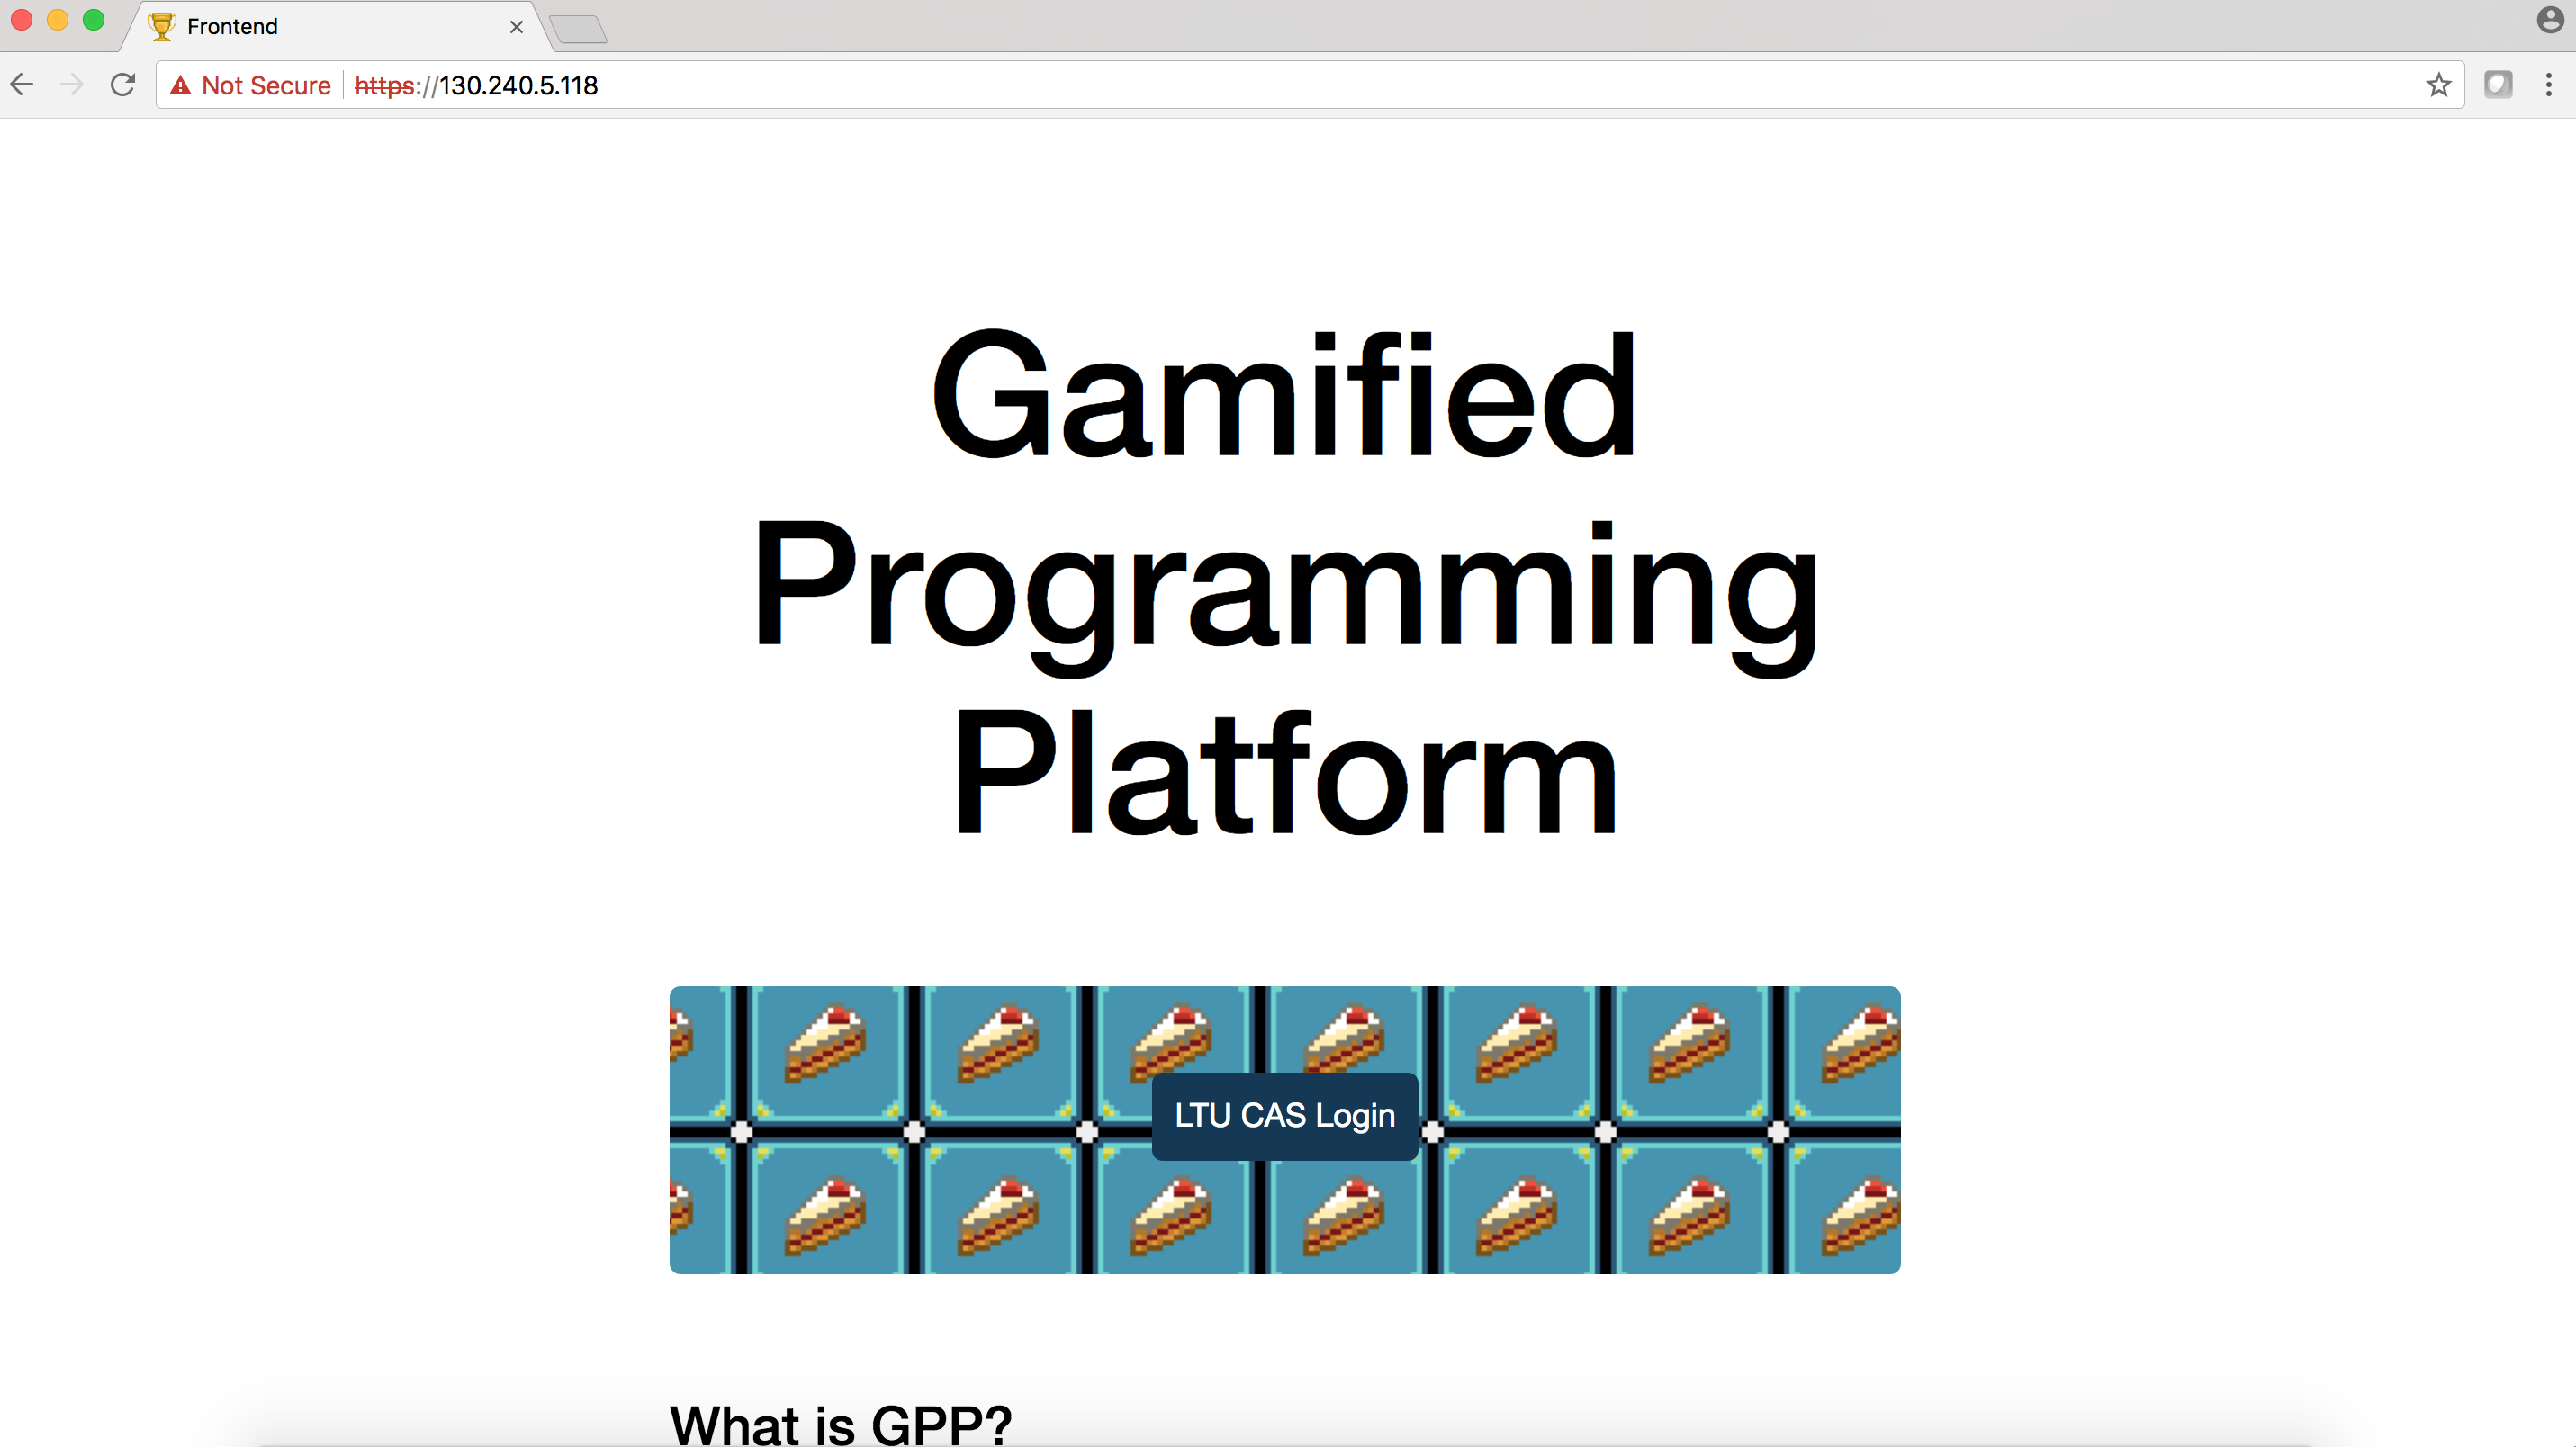
\includegraphics[width=0.8\textwidth]{img/gppinpictures/login2.png}
\caption{Login}
\label{fig:login}
\end{figure}

\begin{figure}[H]
\centering
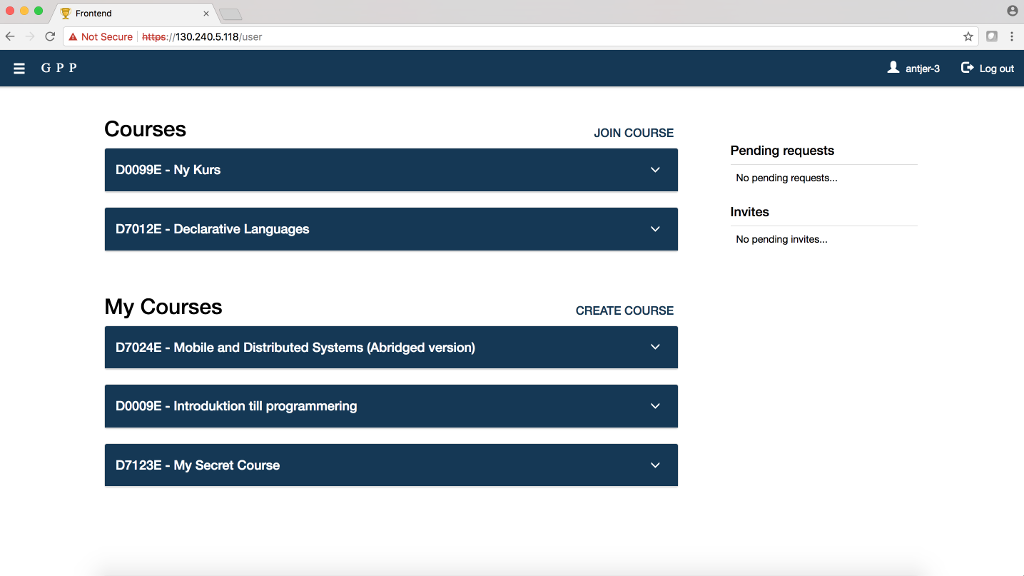
\includegraphics[width=0.8\textwidth]{img/gppinpictures/user.png}
\caption{User page once logged in}
\label{fig:user}
\end{figure}

\begin{figure}[H]
\centering
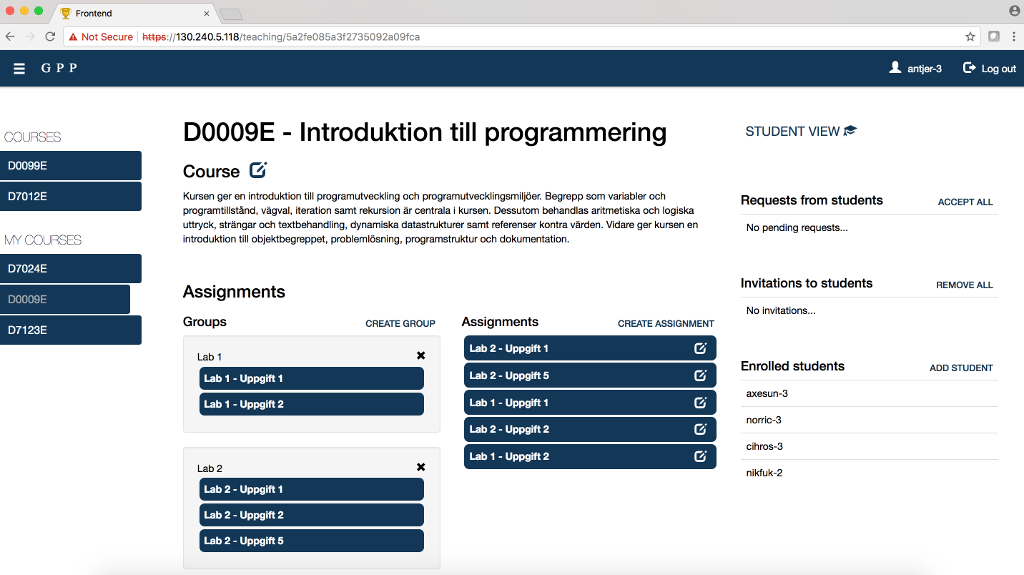
\includegraphics[width=0.8\textwidth]{img/gppinpictures/teacher.png}
\caption{Teacher view for a course}
\label{fig:teacher}
\end{figure}

\begin{figure}[H]
\centering
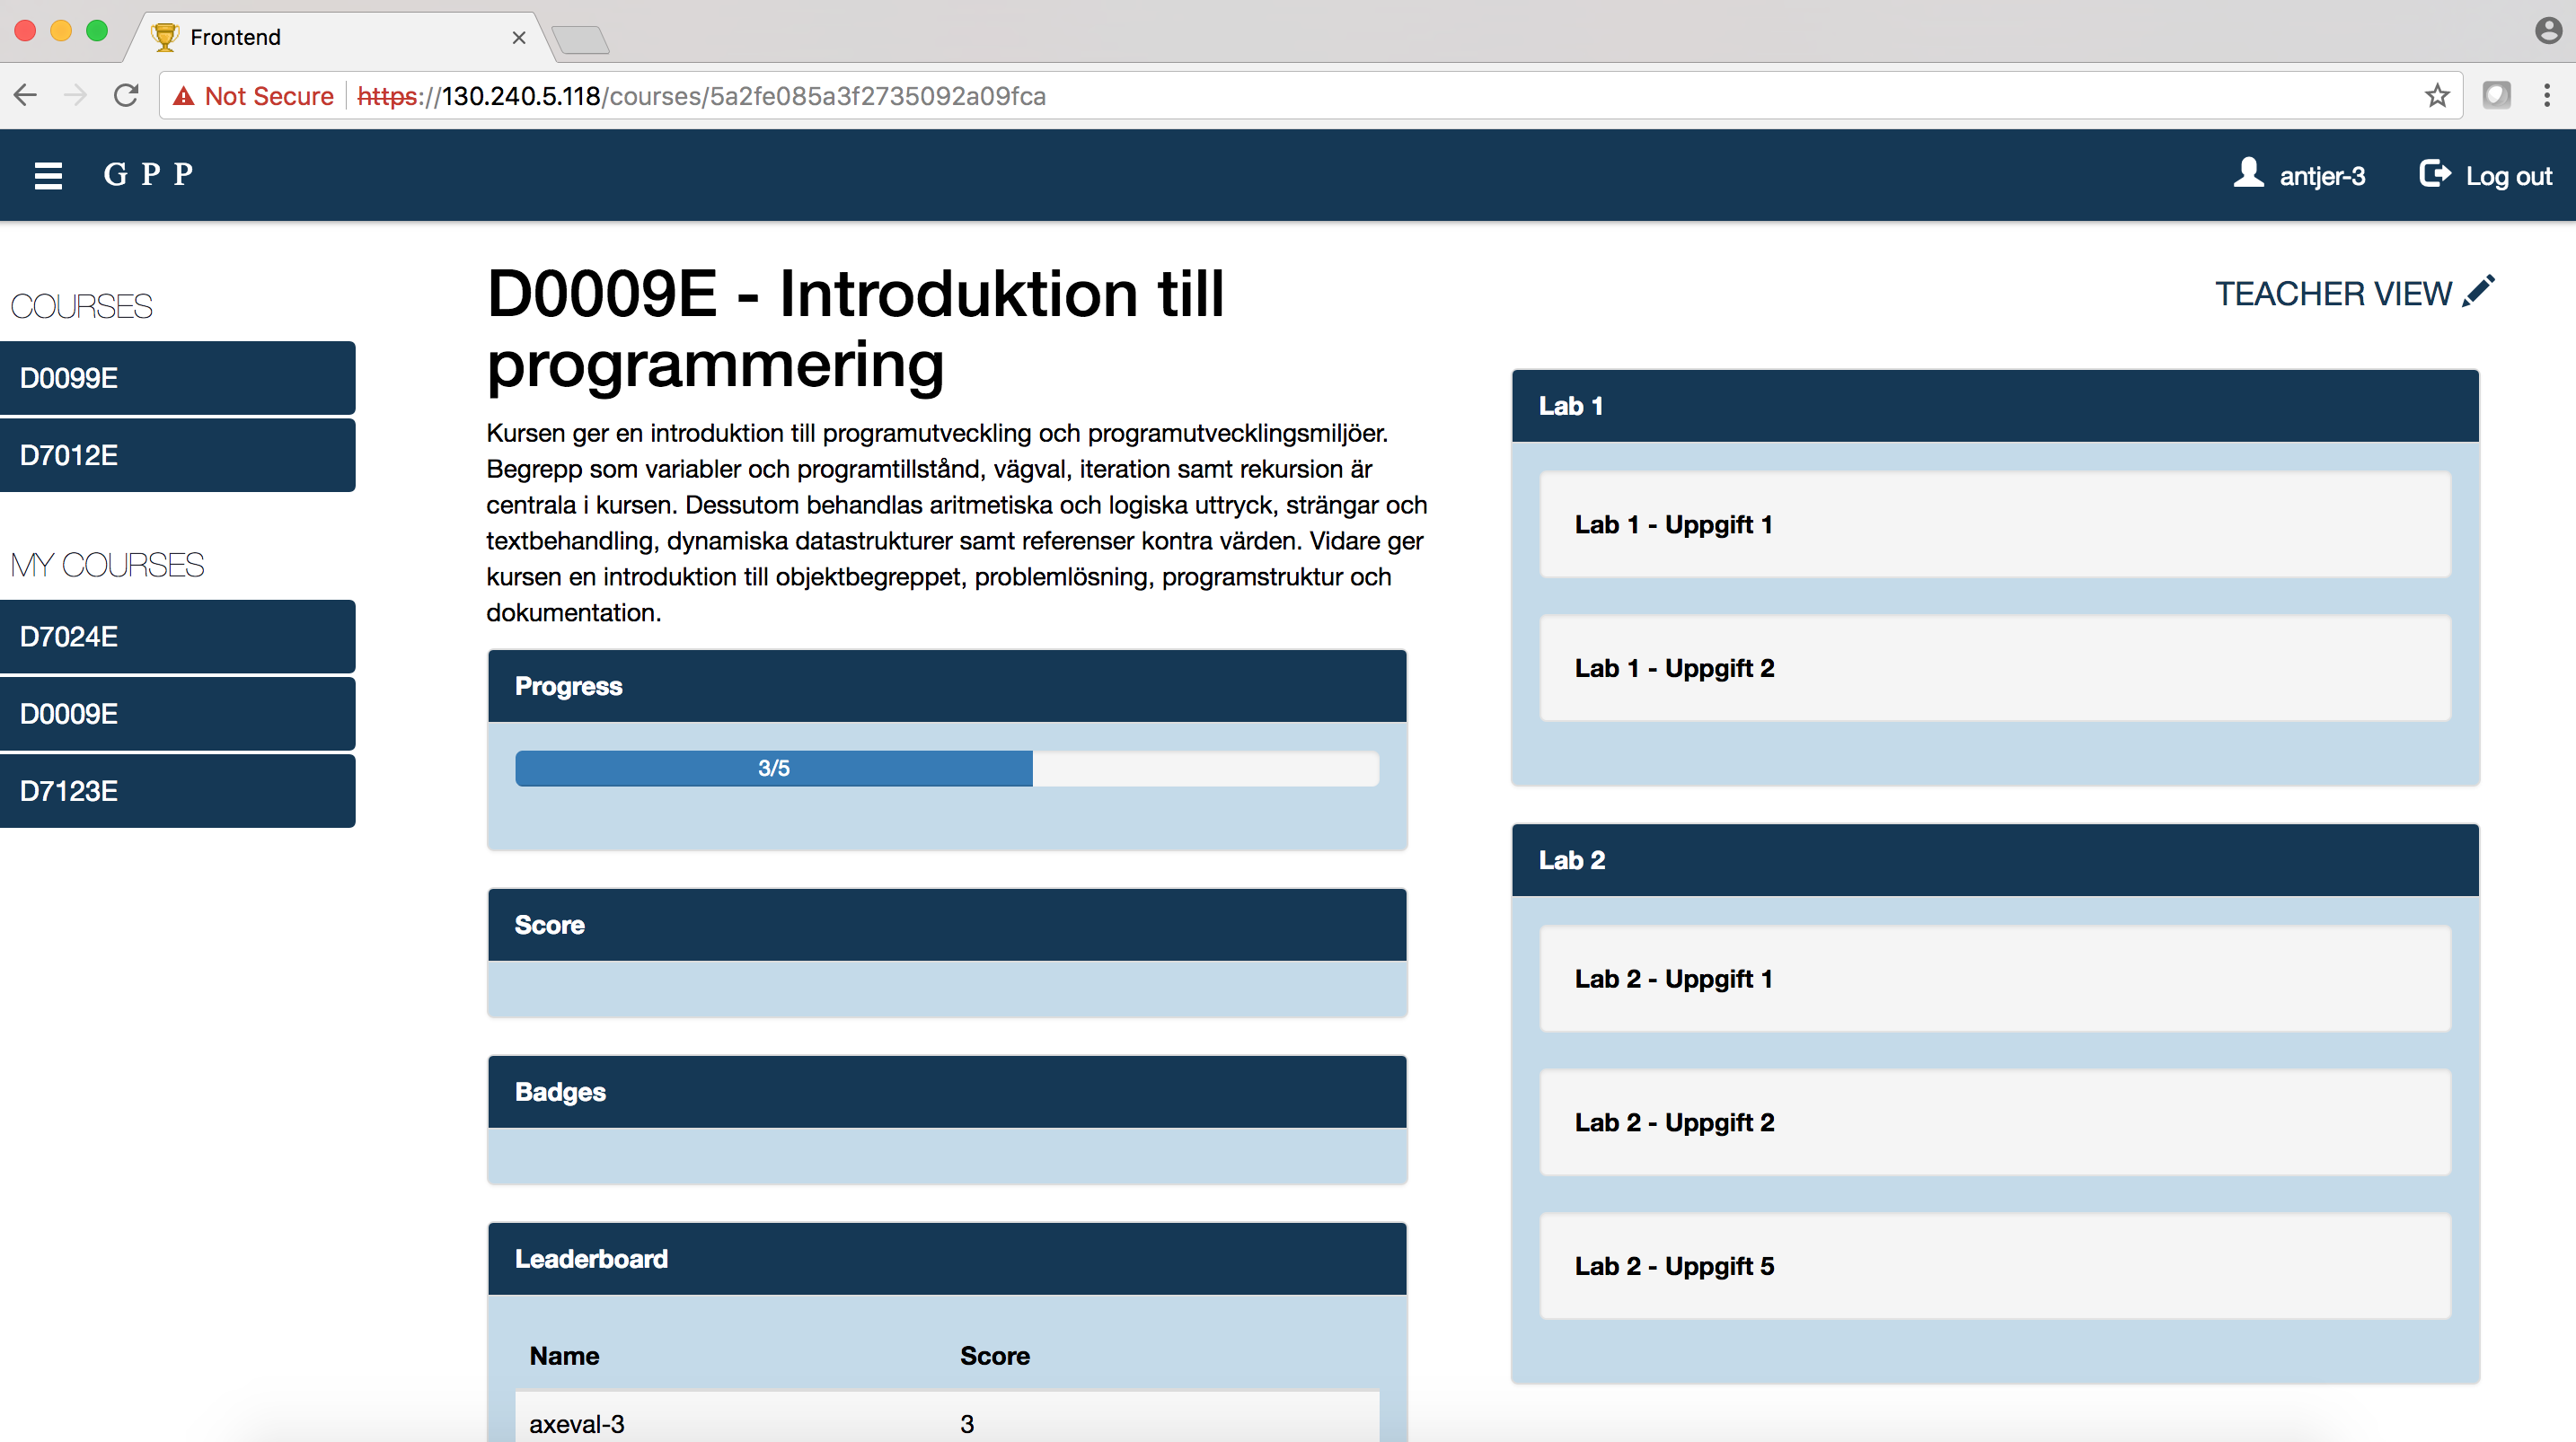
\includegraphics[width=0.8\textwidth]{img/gppinpictures/studentview.png}
\caption{Student view for a course}
\label{fig:student}
\end{figure}

\begin{figure}[H]
\centering
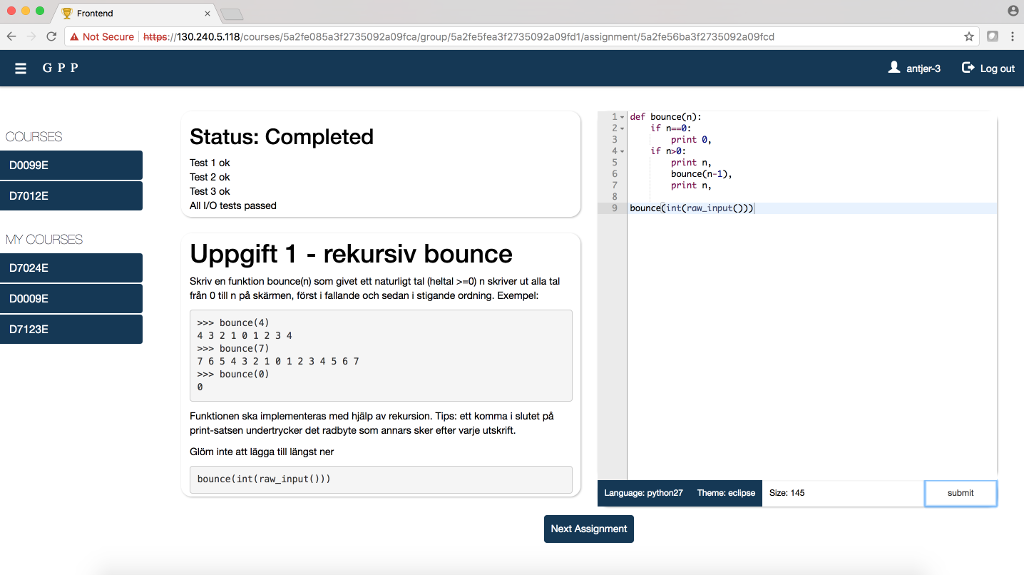
\includegraphics[width=0.8\textwidth]{img/gppinpictures/assignment.png}
\caption{Assignment page}
\label{fig:assignment}
\end{figure}

\begin{figure}[H]
\centering
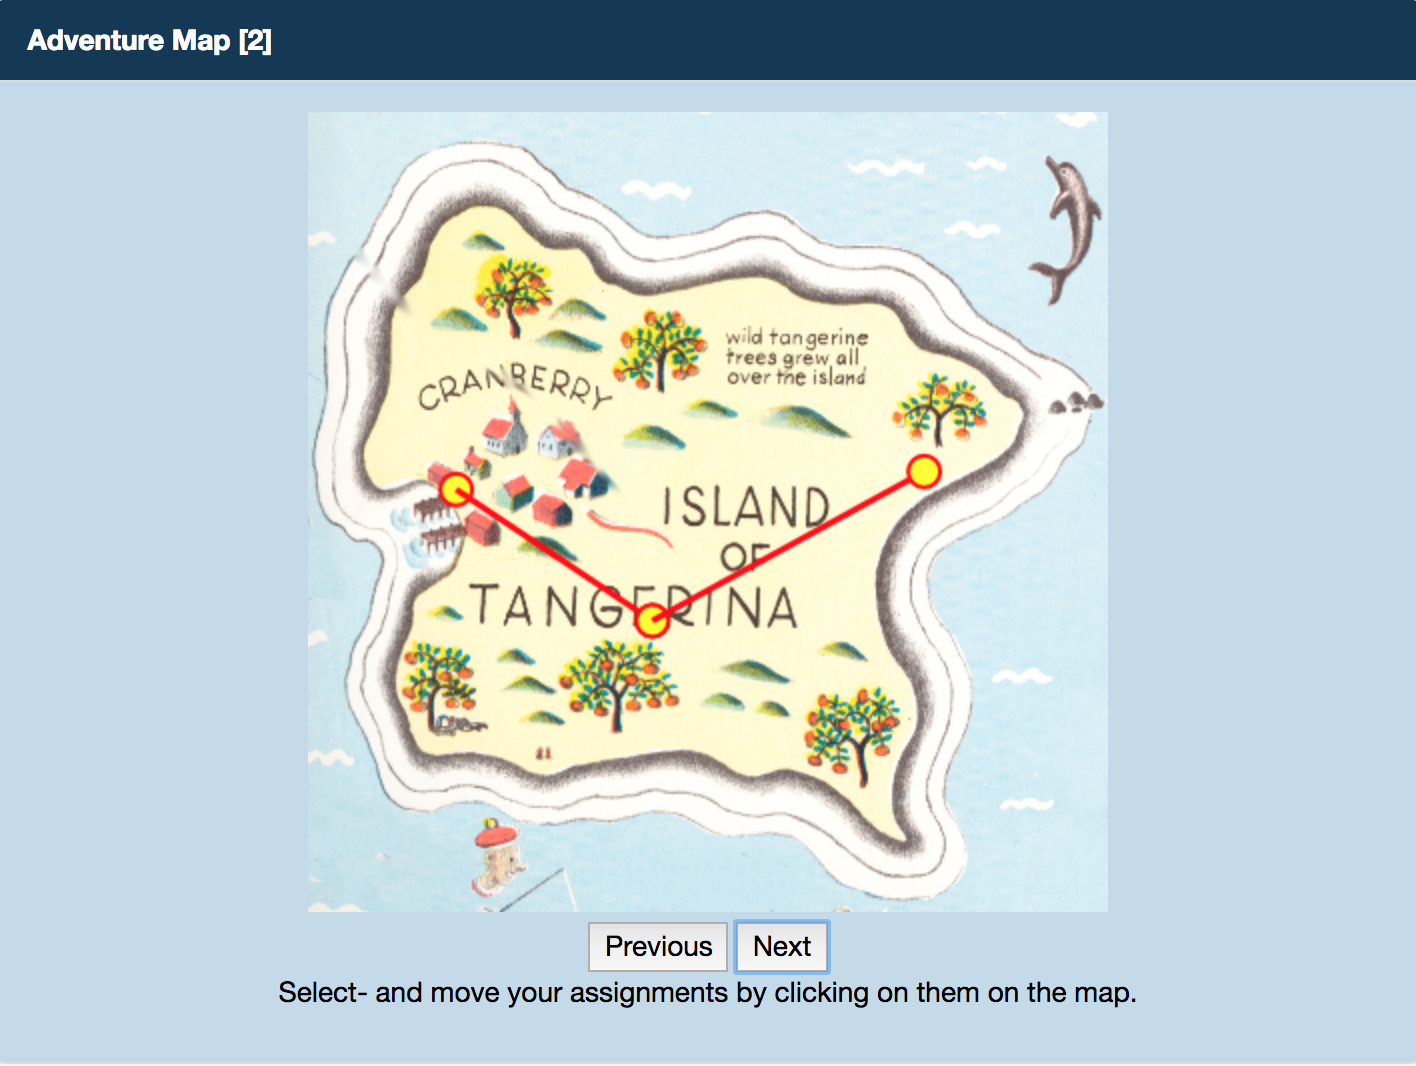
\includegraphics[width=0.8\textwidth]{img/gppinpictures/adventuremap.png}
\caption{Adventure map with assignments}
\label{fig:adventuremap}
\end{figure}

\begin{figure}[H]
\centering
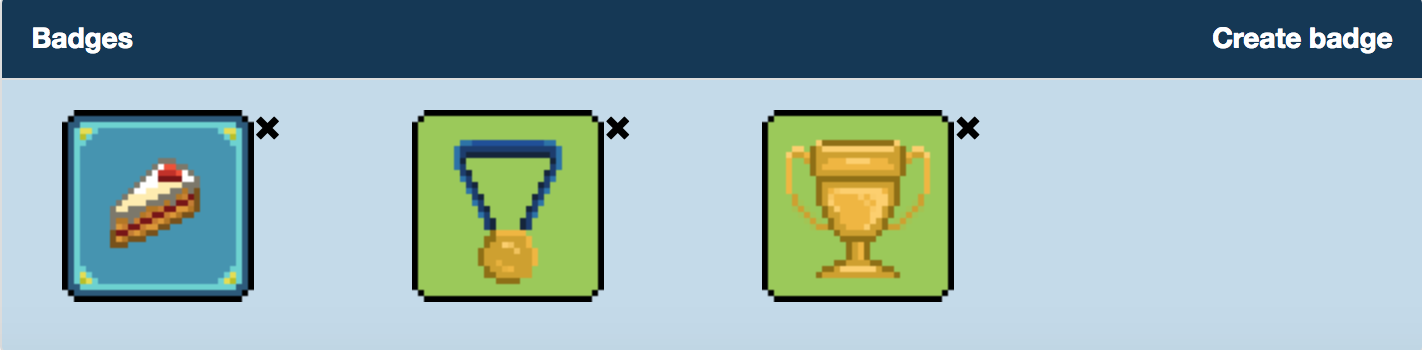
\includegraphics[width=0.8\textwidth]{img/gppinpictures/badges.png}
\caption{Course badges}
\label{fig:login}
\end{figure}

\begin{figure}[H]
\centering
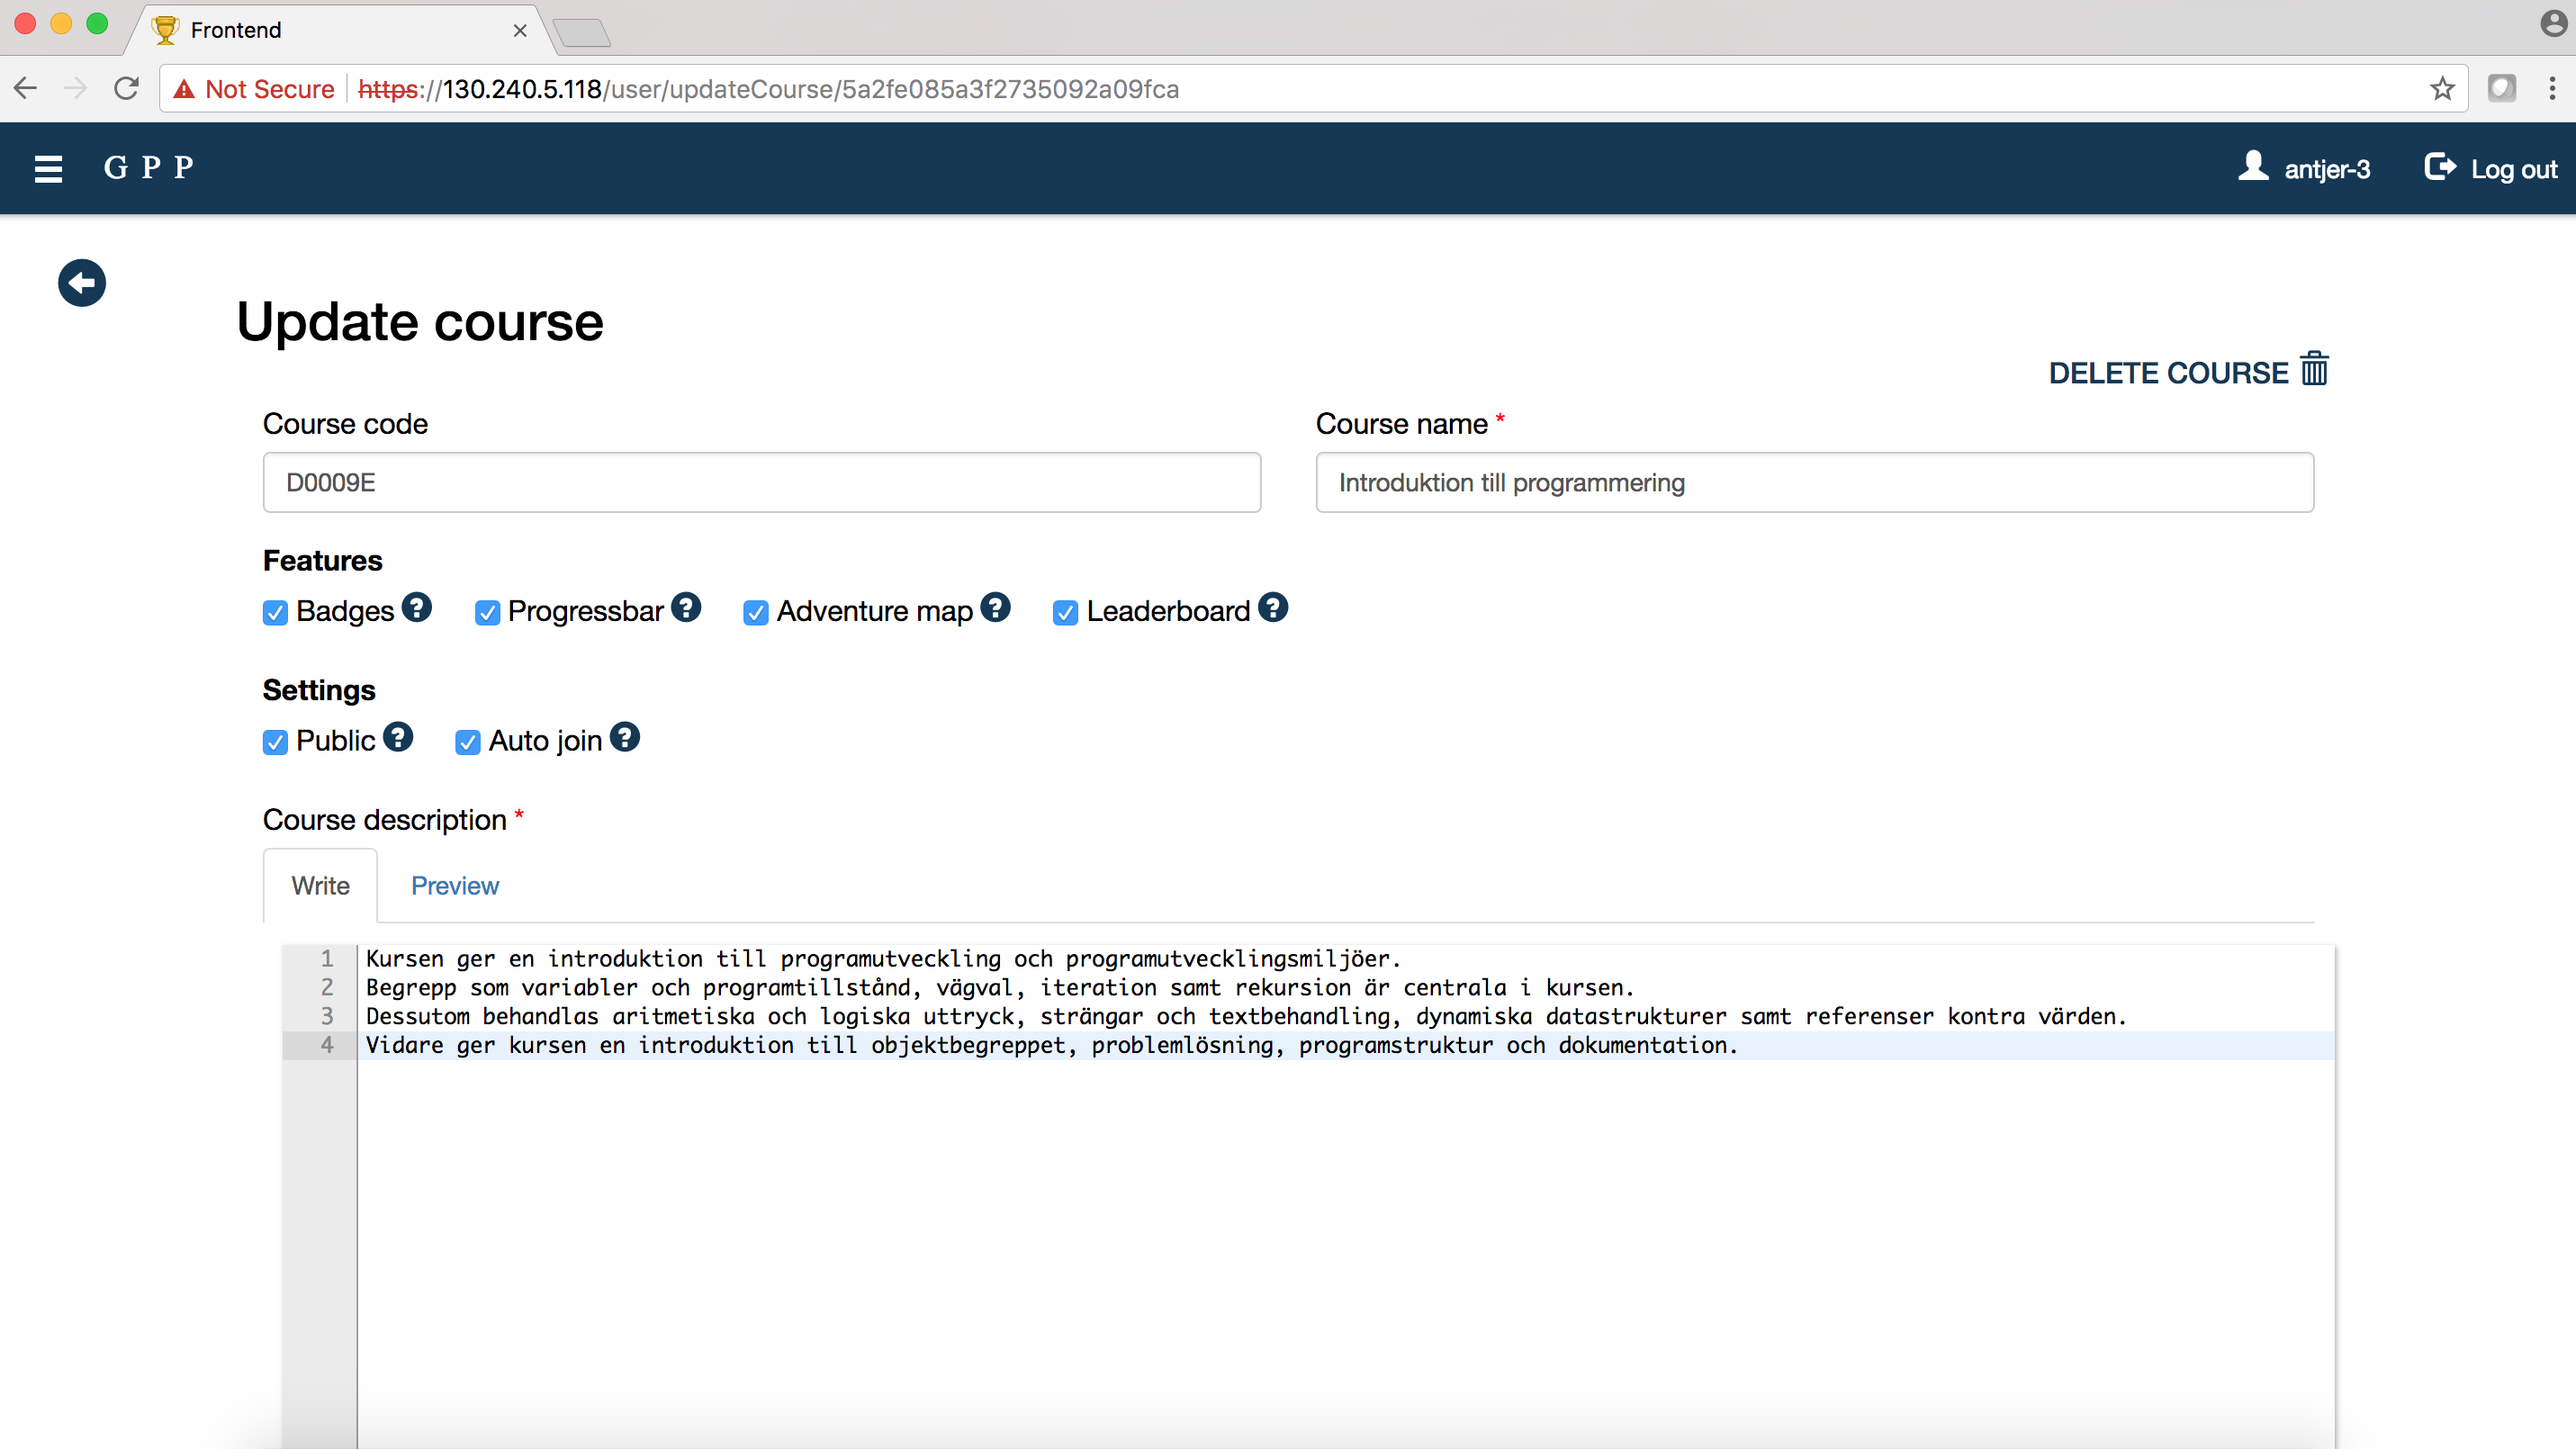
\includegraphics[width=0.8\textwidth]{img/gppinpictures/editcourse.png}
\caption{Edit/create course page}
\label{fig:editcourse}
\end{figure}

\begin{figure}[H]
\centering
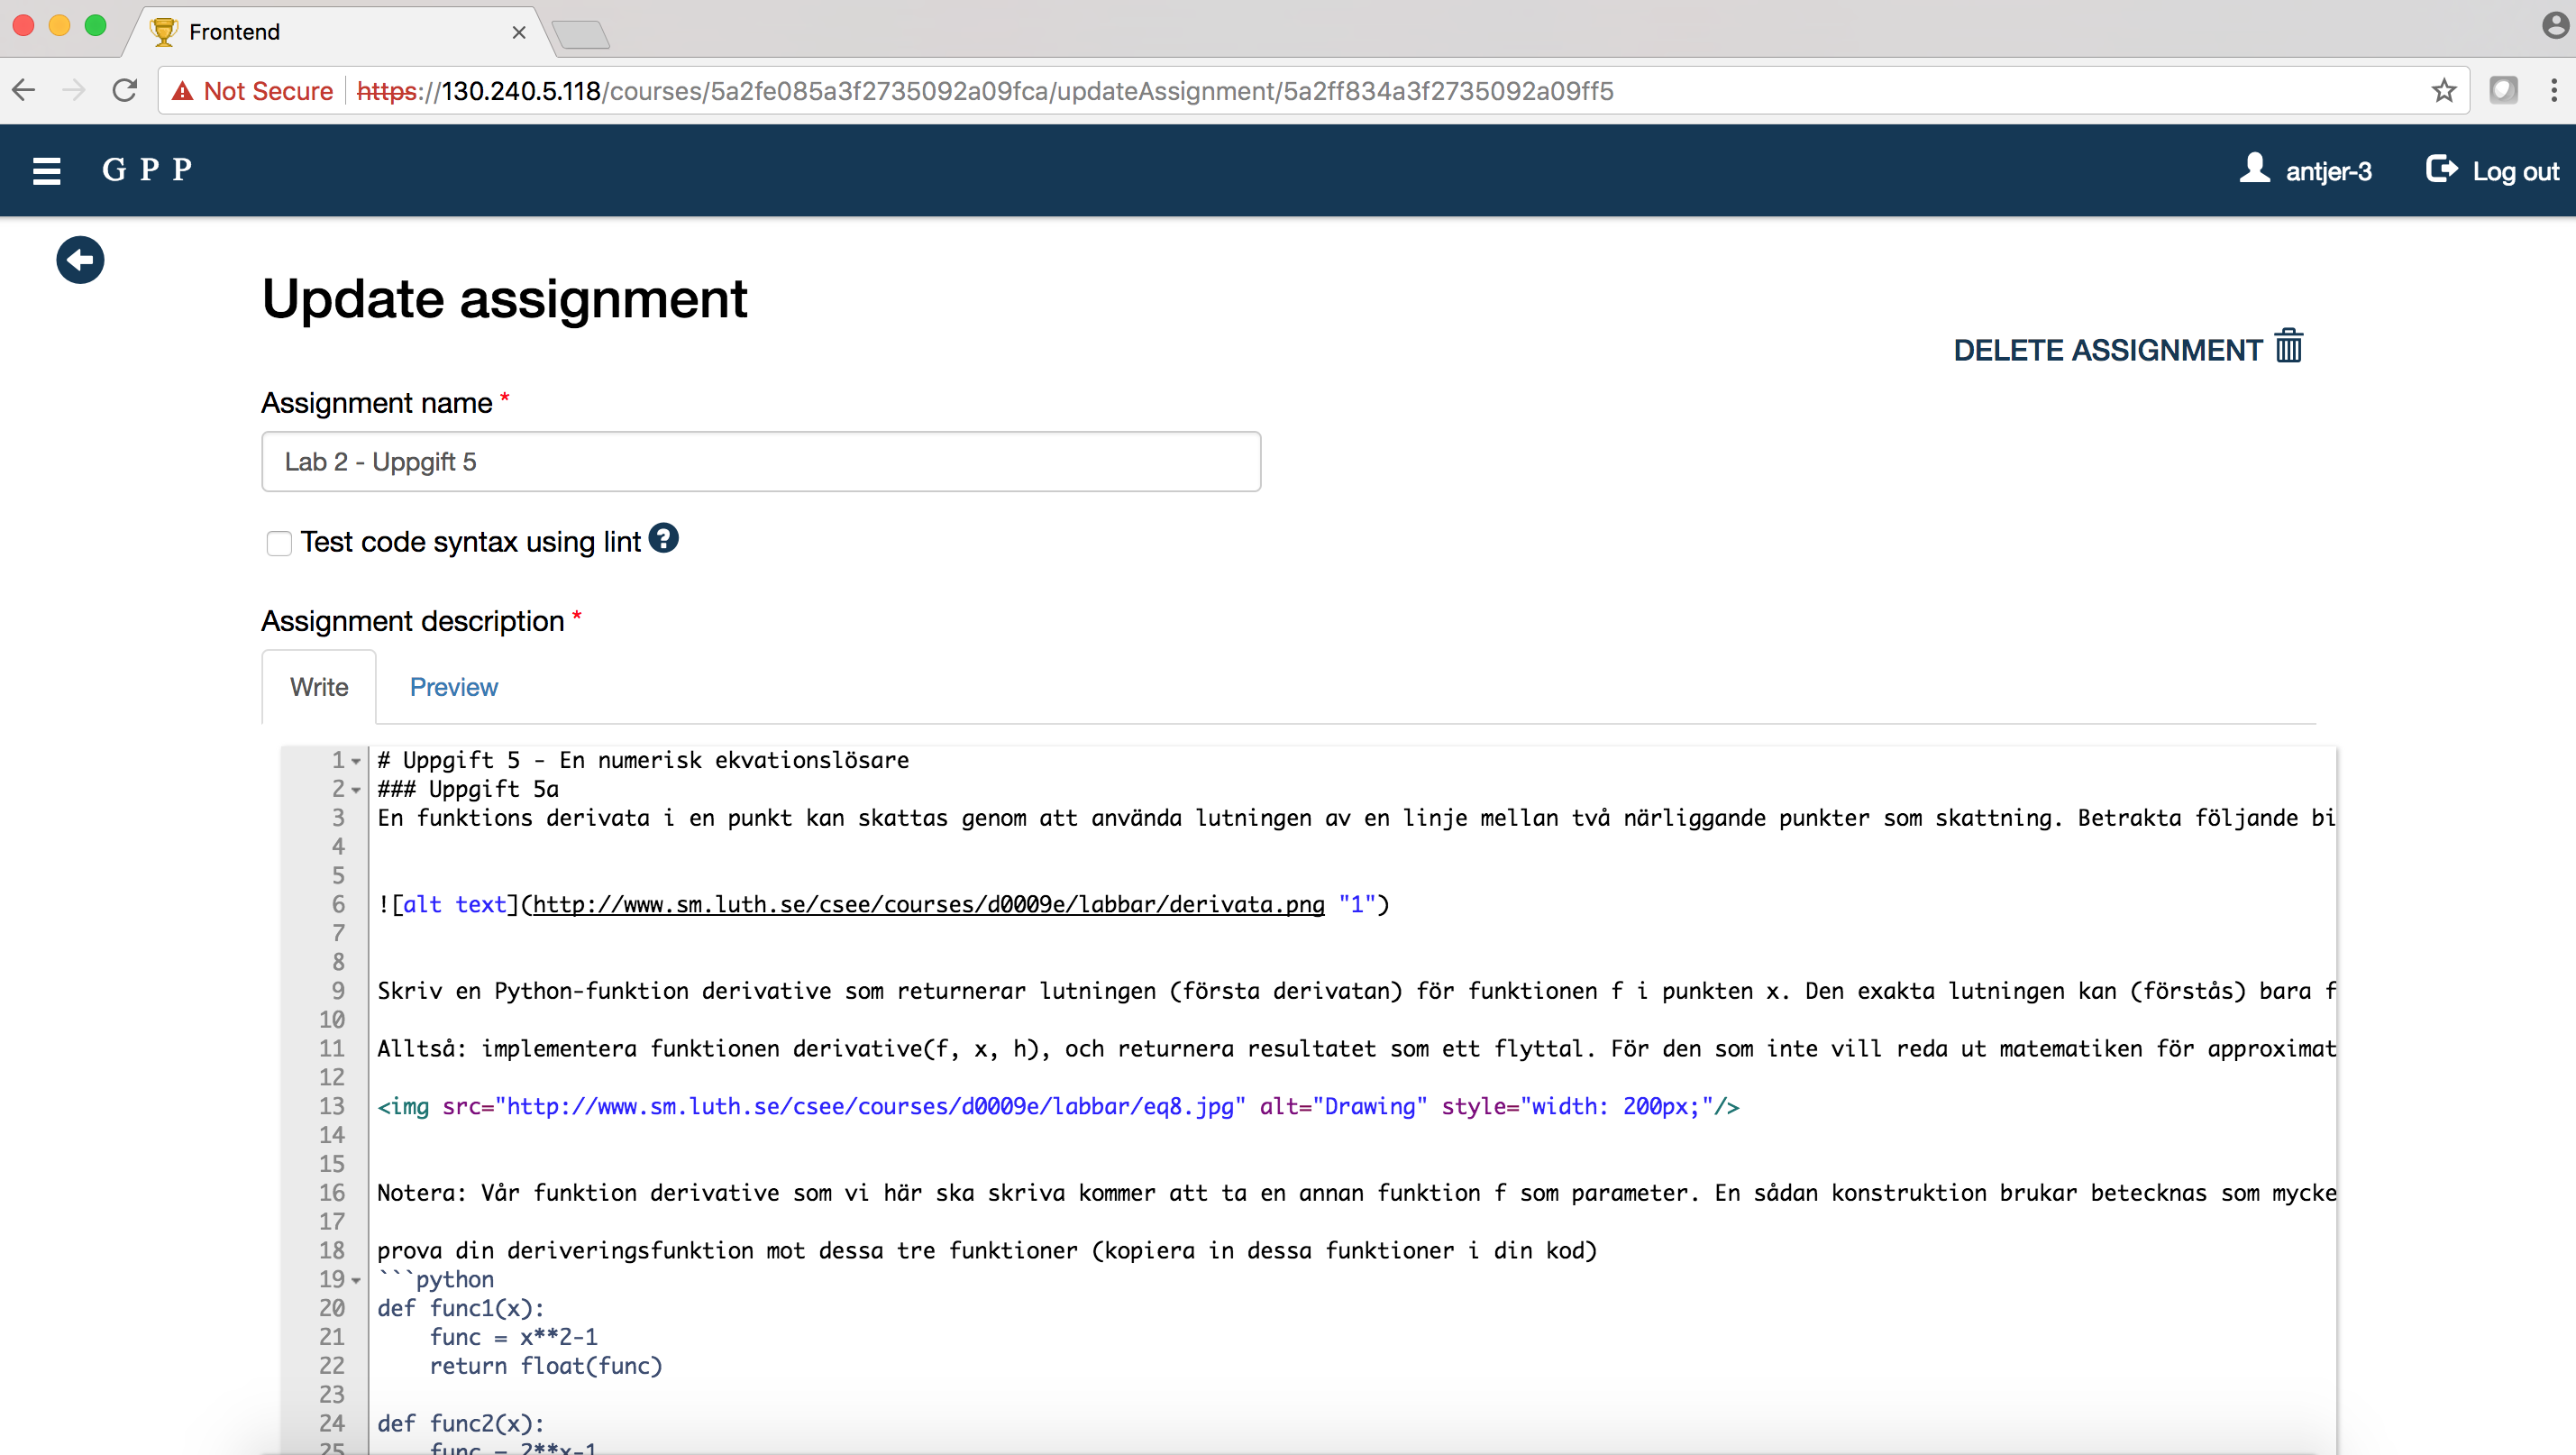
\includegraphics[width=0.8\textwidth]{img/gppinpictures/editassignment.png}
\caption{Edit/create assignment page}
\label{fig:editassignment}
\end{figure}

\begin{figure}[H]
\centering
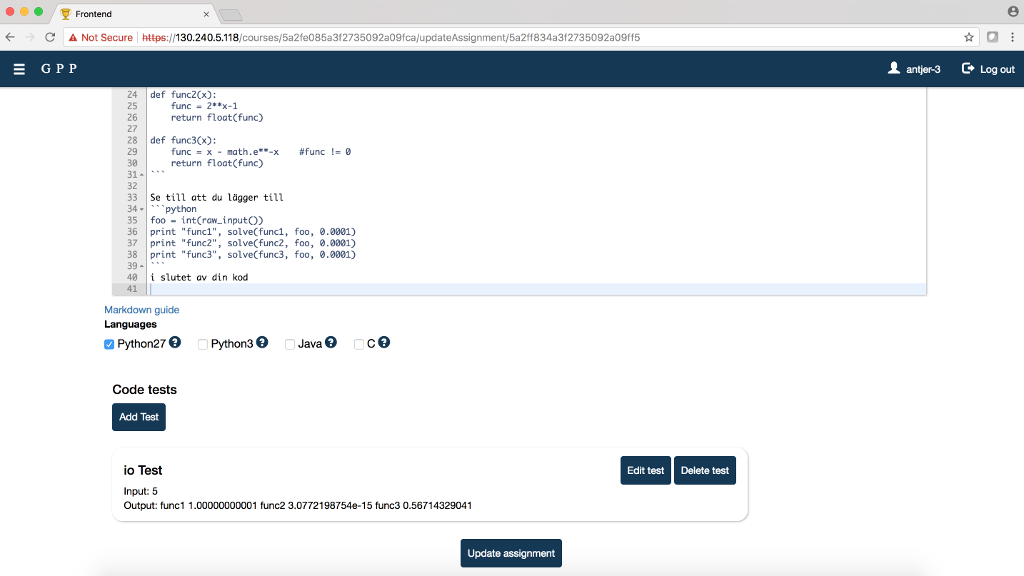
\includegraphics[width=0.8\textwidth]{img/gppinpictures/editassignmenttests.png}
\caption{Tests and language selection for edit/create assignment}
\label{fig:editassignment2}
\end{figure}

\begin{figure}[H]
\centering
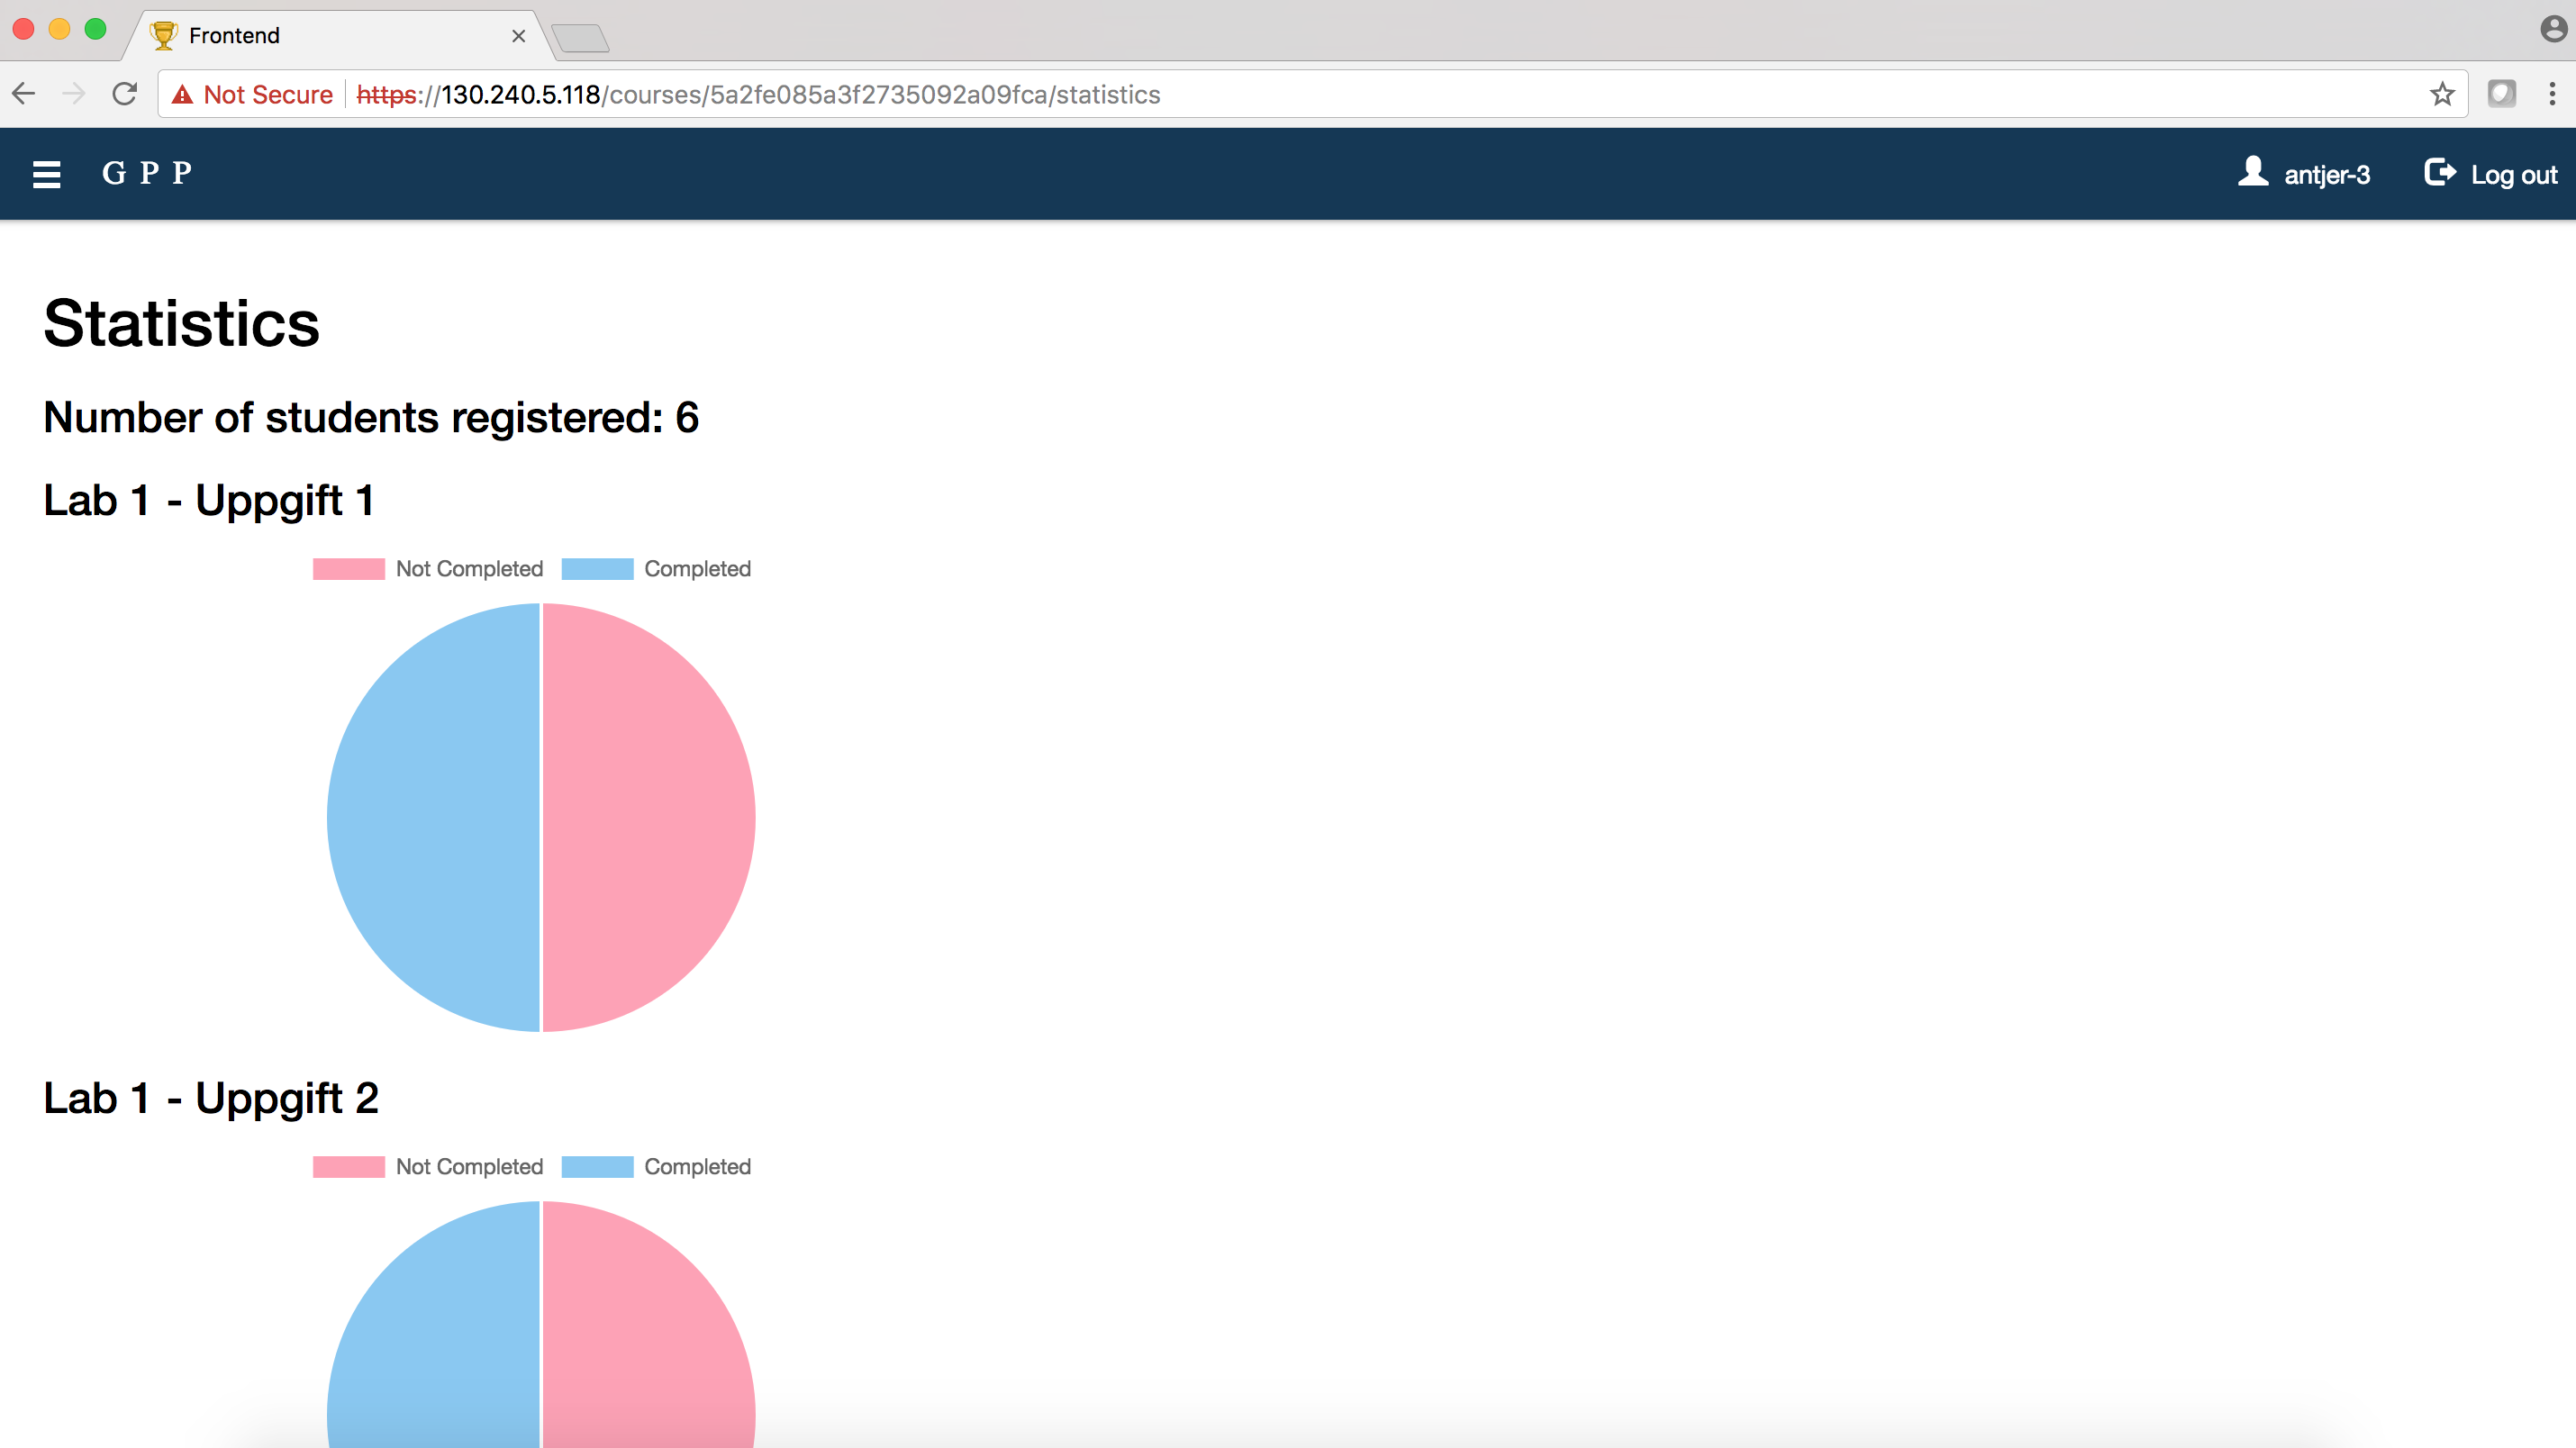
\includegraphics[width=0.8\textwidth]{img/gppinpictures/statistics.png}
\caption{Course statistics page}
\label{fig:statistics}
\end{figure}



\addtocontents{toc}{\protect\end{multicols}}

\end{document}
